\documentclass[12pt]{article}

\usepackage{multirow}
\usepackage{tabularx}
\newcolumntype{Y}{>{\centering\arraybackslash}X}
\usepackage[table,xcdraw]{xcolor}
\usepackage[pdftex]{graphicx}


\usepackage{seqsplit}
\usepackage{url}
\usepackage{import}
\usepackage{longtable}
\usepackage{hyperref}

\makeatletter
\g@addto@macro\UrlSpecials{\camelurl}
\def\camelurl{%
\count@`a
\loop
\mathcode\count@"8000
\uccode`\~\count@\uppercase{\edef~{\mathchar\the\count@\noexpand\breakifupper}}%
\ifnum\count@<`\z
\advance\count@\@ne
\repeat}

\def\breakifupper#1{%
\ifcat .\noexpand#1%
\ifnum`#1>40
\ifnum`#1<91
\penalty\z@
\fi\fi\fi
#1%
}

\makeatother

\pagestyle{plain}
\setcounter{secnumdepth}{2}

\topmargin=0cm
\oddsidemargin=0cm
\textheight=22.0cm
\textwidth=17cm
\parindent=0cm
\parskip=0.15cm
\topskip=0truecm
\raggedbottom
\abovedisplayskip=3mm
\belowdisplayskip=3mm
\abovedisplayshortskip=0mm
\belowdisplayshortskip=2mm
\normalbaselineskip=12pt
\normalbaselines

% environment slightly edited from https://tex.stackexchange.com/questions/10293/latex-template-for-use-cases
\newcommand\tabularhead[1]{
    \begin{table}[ht]
        \addtocounter{use case ID}{1}
        \caption{Use Case \arabic{use case ID} - #1}
        \vspace{0.2cm}
        \begin{tabular}{|p{0.2\linewidth}|p{0.70\linewidth}|}
            \hline
            \textbf{Action} & \textbf{#1} \\
            \hline}

        \newcommand\addrow[2]{#1 & #2\\ \hline}

            \newcommand\addmulrow[2]{ \begin{minipage}[t][][t]{2.5cm}#1\end{minipage}
                &\begin{minipage}[t][][t]{11cm}
                    \begin{enumerate}[itemsep=-1ex] #2   \end{enumerate}
                \end{minipage}\vfill\\ \hline}

            \newenvironment{usecase}{\tabularhead}
        {\hline\end{tabular}\end{table}}



        % cheaty non-functional requirement env

        \newcounter{req ID}
        \newcommand\tabularheadfsd[1]{
            \begin{table}[ht]
                \addtocounter{req ID}{1}
                \caption{Non-Functional Requirement \arabic{req ID} - #1}
                \vspace{0.2cm}
                \begin{tabular}{|p{0.2\linewidth}|p{0.70\linewidth}|}
                    \hline
                    \textbf{Action} & \textbf{#1} \\
                    \hline}

                \newenvironment{requirement}{\tabularheadfsd}
                {\hline\end{tabular}\end{table}}

                \begin{document}

                \vspace*{0.5in}
                \centerline{\bf\Large COMP 354}
                \centerline{\bf\Large Test Document for the project myMoney}

                \vspace*{0.5in}
                \centerline{\bf\Large Team PA-PK}

                \vspace*{0.5in}
                \centerline{\today}

                \vspace*{1.5in}
                \begin{table}[htbp]
                    \caption{Team}
                    \begin{center}
                        \begin{tabular}{|r | c|}
                            \hline
                            Name & ID Number \\
                            \hline\hline
                            Anne-Laure Ehresmann & 27858906 \\
                            \hline
                            Marc-Antoine Dube & 40029307 \\
                            \hline
                            Kadeem Caines & 26343600 \\
                            \hline
                            Abdel Rahman Jawhar & 27192142 \\
                            \hline
                            Keith Dion & 40036340 \\
                            \hline
                            Hrachya Hakobyan & 40041555 \\
                            \hline
                            Andrew-Smith & 40034936 \\
                            \hline
                            Dongyu Chen & 27241909 \\
                            \hline
                            Yauheni Karaniuk & 40005680 \\
                            \hline
                            Renny Xu & 40005262\\
                            \hline
                            Wei Wang & 40041116 \\
                            \hline
                        \end{tabular}
                    \end{center}
                \end{table}

                \begin{table}[htbp]
                    \caption{Revision history}
                    \begin{center}
                        \begin{tabular}{|r | c| c |}
                            \hline
                            Version & Date & Changes \\
                            \hline
                            1.0 & 15 March 2018 & Completed test document \\
                            \hline
                        \end{tabular}
                    \end{center}
                \end{table}


                \tableofcontents
\listoffigures
\clearpage

\clearpage

\section{Introduction}

The aim of this document is to ensure that a coherent and accurate testing strategy is used by the testing team. It looks at the implementation of the system described in the Design Plan, test its validity, robustness, and reliableness as a software, as well as ensuring that the requirements in the Requirements Specification are met. It seeks to do this in a rigorous and justified manner.
This document contains an overarching test plan, which seeks to outline each test subsystem, their strategy with regards to testing the associated requirements, and their execution strategy. This document then contains, for each subsystem, a detailed explanation of the set of tests included, and a test case for each individual test. Put together, the test subsystems group into a entire system test.

\section{Test Plan}

The system test plan has been split into five subsystem tests:

\begin{itemize}
    \item \textbf{Functional Testing:} This test subsystem seeks to certify the functionality of the software against the use cases in the Requirements Specification. This category will use black-box testing as its strategy, verifying the usability given different inputs and regardless of the implementation of the sfotware. In its execution, a developer running such a test will typically first identify how the software should perform the functionality to be tested, in the given use case scenario. Then, he or she verifies the functionality, behaviour, and reliability of the software given valid user behaviour, and then checks for robustness given exceptional situations.
    \item \textbf{Structural Testing:} This test subsystem seeks to verify the structure and code logic of the software. We ensure here that each part of the code functions as expected given both valid and invalid input, and test the behaviour of the system in unexpected states. This will let us confirm the validity of the code flow, and ensure logic faults are caught. For the execution of the test, we will use JUnit to create individual tests for each case. Each test will have an initial setup phase, a test phase, and a teardown phase, to ensure independence of state between each test. A test will also use Mockito, a mocking library, to ensure that the failure of some other, unrelated component of the code does not affect the performance of the tested component in each test.
    \item \textbf{Performance Testing:} This test subsystem seeks to measure the behaviour of the software in extreme states, when under particular workloads or dealing with extremely large datasets. It is useful for testing a number of our non-functional requirements, notably reliability, scalability, and, obviously, performance. In its execution, The tests measure performance statistics given a normal or 'control' environment, then compare it to the performance statistic given a particular dataset or workload.
    \item \textbf{Acceptance Testing:} This test subsystem seeks to meet the requirements set in the Requirements Specification, from the point of the view of a user. This is also a black-box testing category, as in functional testing, but unlike the aforementioned, we are instead performing a validation of the system through the perspective of the user, not the devloper: is our system actually what the user needs? In its execution, the system is given to a user, who will assert whether his needs are met by the system and if it corresponds to how he or she expects the software to function.
    \item \textbf{Installation Testing:} This test subsystem seeks to verify that the installation process is both successful and easy in the platforms to be supported. This means ensuring that the choices taken by the user with regards to installation are respected (location of installation, installation just for one user or for whole computer...), verify that all dependent files and libraries are successfully linked and loaded, and valid configurations and connectivity to the database. The execution of this category is simply an activity wherein the installation process is attempted in a particular environment, testing all decisions and options available in the installation.
\end{itemize}

\section{Functional Testing}

As aforementioned, each test here is directly related to a use case in the requirements document.

\subsubsection{Create User Account}
\begin{longtable}{|m{4cm}|l|l|}
\hline
\cellcolor[HTML]{C0C0C0}\textbf{Test Case} & \multicolumn{2}{p{13cm}|}{First name, last name, username and password are mandatory}\\ \hline
\cellcolor[HTML]{C0C0C0}\textbf{Description} & \multicolumn{2}{p{13cm}|}{The user cannot sign up without providing a valid first name, last name, a username and a password}\\ \hline
\cellcolor[HTML]{C0C0C0}\textbf{Input/Steps} & \multicolumn{2}{p{13cm}|}{\begin{tabular}[c]{@{}l@{}}1. Go to 'Sign Up'\\ 2. Leave all the input fields blank\\ 3. Click 'Sign up'\\ \end{tabular}}\\ \hline
\cellcolor[HTML]{C0C0C0}\textbf{Output/Results} & \multicolumn{2}{p{13cm}|}{\begin{tabular}[c]{@{}l@{}}$\bullet$ Sign up fails, the account is not created\\ $\bullet$ An error window displays all the errors\\ \end{tabular}}\\ \hline
\end{longtable}
\begin{longtable}{|m{4cm}|l|l|}
\hline
\cellcolor[HTML]{C0C0C0}\textbf{Test Case} & \multicolumn{2}{p{13cm}|}{The username must be unique}\\ \hline
\cellcolor[HTML]{C0C0C0}\textbf{Description} & \multicolumn{2}{p{13cm}|}{The user cannot sign up with an already existing username}\\ \hline
\cellcolor[HTML]{C0C0C0}\textbf{Input/Steps} & \multicolumn{2}{p{13cm}|}{\begin{tabular}[c]{@{}l@{}}1. Successfully sign\\ 2. Log out\\ 3. Go to 'Sign up'\\ 4. Fill in all the input fields\\ 5. Set the username field to be the username of the user created in the first step\\ 6. Click 'Sign Up'\\ \end{tabular}}\\ \hline
\cellcolor[HTML]{C0C0C0}\textbf{Output/Results} & \multicolumn{2}{p{13cm}|}{\begin{tabular}[c]{@{}l@{}}$\bullet$ Sign up failed, the account is not created\\ $\bullet$ An error window notifies that the username already exists\\ \end{tabular}}\\ \hline
\end{longtable}
\begin{longtable}{|m{4cm}|l|l|}
\hline
\cellcolor[HTML]{C0C0C0}\textbf{Test Case} & \multicolumn{2}{p{13cm}|}{The password must be valid}\\ \hline
\cellcolor[HTML]{C0C0C0}\textbf{Description} & \multicolumn{2}{p{13cm}|}{The user cannot sign up with a password not matching the required format, as specified in the business rules}\\ \hline
\cellcolor[HTML]{C0C0C0}\textbf{Input/Steps} & \multicolumn{2}{p{13cm}|}{\begin{tabular}[c]{@{}l@{}}1. Go to 'Sign up'\\ 2. Fill in all the input fields\\ 3. Set the password to an alpha-numeric sequence of length less than 4\\ 4. Set the repeat password field to match the password field\\ 5. Click 'Sign Up'\\ \end{tabular}}\\ \hline
\cellcolor[HTML]{C0C0C0}\textbf{Output/Results} & \multicolumn{2}{p{13cm}|}{\begin{tabular}[c]{@{}l@{}}$\bullet$ Sign up failed, the account is not created\\ $\bullet$ An error window notifies that the password is not valid\\ \end{tabular}}\\ \hline
\end{longtable}
\begin{longtable}{|m{4cm}|l|l|}
\hline
\cellcolor[HTML]{C0C0C0}\textbf{Test Case} & \multicolumn{2}{p{13cm}|}{The user account is successfully created}\\ \hline
\cellcolor[HTML]{C0C0C0}\textbf{Description} & \multicolumn{2}{p{13cm}|}{The user must be able to successfully create an account provided that all input information is valid}\\ \hline
\cellcolor[HTML]{C0C0C0}\textbf{Input/Steps} & \multicolumn{2}{p{13cm}|}{\begin{tabular}[c]{@{}l@{}}1. Go to 'Sign up'\\ 2. Fill in all the input fields with valid data\\ 3. Click 'Sign Up'\\ 4. Moved to the login page: input the username and the passowrd\\ 5. Click 'Login'\\ \end{tabular}}\\ \hline
\cellcolor[HTML]{C0C0C0}\textbf{Output/Results} & \multicolumn{2}{p{13cm}|}{\begin{tabular}[c]{@{}l@{}}$\bullet$ Sign up successful, the account is created\\ $\bullet$ The user is logged-in to the newly created account\\ \end{tabular}}\\ \hline
\end{longtable}

\subsubsection{Delete User Account}
\begin{longtable}{|m{4cm}|l|l|}
\hline
\cellcolor[HTML]{C0C0C0}\textbf{Test Case} & \multicolumn{2}{p{13cm}|}{Password required}\\ \hline
\cellcolor[HTML]{C0C0C0}\textbf{Description} & \multicolumn{2}{p{13cm}|}{The program asks for the user's password before to delete the account}\\ \hline
\cellcolor[HTML]{C0C0C0}\textbf{Input/Steps} & \multicolumn{2}{p{13cm}|}{\begin{tabular}[c]{@{}l@{}}1. Go to 'Update User Account'\\ 2. Click 'Delete user'\\ \end{tabular}}\\ \hline
\cellcolor[HTML]{C0C0C0}\textbf{Output/Results} & \multicolumn{2}{p{13cm}|}{\begin{tabular}[c]{@{}l@{}}$\bullet$ A an input window appears asking for the user password\\ \end{tabular}}\\ \hline
\end{longtable}
\begin{longtable}{|m{4cm}|l|l|}
\hline
\cellcolor[HTML]{C0C0C0}\textbf{Test Case} & \multicolumn{2}{p{13cm}|}{The password must be valid}\\ \hline
\cellcolor[HTML]{C0C0C0}\textbf{Description} & \multicolumn{2}{p{13cm}|}{The user cannot delete the account if the password is invalid}\\ \hline
\cellcolor[HTML]{C0C0C0}\textbf{Input/Steps} & \multicolumn{2}{p{13cm}|}{\begin{tabular}[c]{@{}l@{}}1. Go to 'Update User Account'\\ 2. Click 'Delete user'\\ 3. Enter a wrong password\\ \end{tabular}}\\ \hline
\cellcolor[HTML]{C0C0C0}\textbf{Output/Results} & \multicolumn{2}{p{13cm}|}{\begin{tabular}[c]{@{}l@{}}$\bullet$ The account is not deleted\\ $\bullet$ An error window must appear notifying the user that the password was invalid\\ \end{tabular}}\\ \hline
\end{longtable}
\begin{longtable}{|m{4cm}|l|l|}
\hline
\cellcolor[HTML]{C0C0C0}\textbf{Test Case} & \multicolumn{2}{p{13cm}|}{The account is successfully deleted}\\ \hline
\cellcolor[HTML]{C0C0C0}\textbf{Description} & \multicolumn{2}{p{13cm}|}{The user account is successfully deleted if the password is correct}\\ \hline
\cellcolor[HTML]{C0C0C0}\textbf{Input/Steps} & \multicolumn{2}{p{13cm}|}{\begin{tabular}[c]{@{}l@{}}1. Go to 'Update User Account'\\ 2. Click 'Delete user'\\ 3. Enter the correct password\\ \end{tabular}}\\ \hline
\cellcolor[HTML]{C0C0C0}\textbf{Output/Results} & \multicolumn{2}{p{13cm}|}{\begin{tabular}[c]{@{}l@{}}$\bullet$ The account is not deleted\\ $\bullet$ An error window must appear notifying the user that the password was invalid\\ \end{tabular}}\\ \hline
\end{longtable}
\begin{longtable}{|m{4cm}|l|l|}
\hline
\cellcolor[HTML]{C0C0C0}\textbf{Test Case} & \multicolumn{2}{p{13cm}|}{The user account is successfully created}\\ \hline
\cellcolor[HTML]{C0C0C0}\textbf{Description} & \multicolumn{2}{p{13cm}|}{The user must be able to successfully create an account provided that all input information is valid}\\ \hline
\cellcolor[HTML]{C0C0C0}\textbf{Input/Steps} & \multicolumn{2}{p{13cm}|}{\begin{tabular}[c]{@{}l@{}}1. Go to 'Sign up'\\ 2. Fill in all the input fields with valid data\\ 3. Click 'Sign Up'\\ 4. Moved to the login page: input the username and the passowrd\\ 5. Click 'Login'\\ \end{tabular}}\\ \hline
\cellcolor[HTML]{C0C0C0}\textbf{Output/Results} & \multicolumn{2}{p{13cm}|}{\begin{tabular}[c]{@{}l@{}}$\bullet$ Sign up successful, the account is created\\ $\bullet$ The user is logged-in to the newly created account\\ \end{tabular}}\\ \hline
\end{longtable}

\subsubsection{Add Bank Account to a User Account}
\begin{longtable}{|m{4cm}|l|l|}
\hline
\cellcolor[HTML]{C0C0C0}\textbf{Test Case} & \multicolumn{2}{p{13cm}|}{Add a valid bank account to a user}\\ \hline
\cellcolor[HTML]{C0C0C0}\textbf{Description} & \multicolumn{2}{p{13cm}|}{A valid bank account should be added to the user}\\ \hline
\cellcolor[HTML]{C0C0C0}\textbf{Input/Steps} & \multicolumn{2}{p{13cm}|}{\begin{tabular}[c]{@{}l@{}}1. Go to the main screen\\ 2. Input an account ID in the 'Enter Account ID' field\\ 3. Click the 'Add' button\\ \end{tabular}}\\ \hline
\cellcolor[HTML]{C0C0C0}\textbf{Output/Results} & \multicolumn{2}{p{13cm}|}{\begin{tabular}[c]{@{}l@{}}$\bullet$ A row should be added in the table of account\\ \end{tabular}}\\ \hline
\end{longtable}
\begin{longtable}{|m{4cm}|l|l|}
\hline
\cellcolor[HTML]{C0C0C0}\textbf{Test Case} & \multicolumn{2}{p{13cm}|}{Add a same account to a user}\\ \hline
\cellcolor[HTML]{C0C0C0}\textbf{Description} & \multicolumn{2}{p{13cm}|}{An account should not be added to the same user twice}\\ \hline
\cellcolor[HTML]{C0C0C0}\textbf{Input/Steps} & \multicolumn{2}{p{13cm}|}{\begin{tabular}[c]{@{}l@{}}1. Go to the main screen\\ 2. Input an account ID in the 'Enter Account ID' field\\ 3. Click the 'Add' button\\ \end{tabular}}\\ \hline
\cellcolor[HTML]{C0C0C0}\textbf{Output/Results} & \multicolumn{2}{p{13cm}|}{\begin{tabular}[c]{@{}l@{}}$\bullet$ Failure, the account is not added\\ $\bullet$ An error window displays all the errors\\ \end{tabular}}\\ \hline
\end{longtable}
\begin{longtable}{|m{4cm}|l|l|}
\hline
\cellcolor[HTML]{C0C0C0}\textbf{Test Case} & \multicolumn{2}{p{13cm}|}{Add an account used by another user}\\ \hline
\cellcolor[HTML]{C0C0C0}\textbf{Description} & \multicolumn{2}{p{13cm}|}{An account used by another user should not be added to another user}\\ \hline
\cellcolor[HTML]{C0C0C0}\textbf{Input/Steps} & \multicolumn{2}{p{13cm}|}{\begin{tabular}[c]{@{}l@{}}1. Go to the main screen\\ 2. Input an account ID in the 'Enter Account ID' field\\ 3. Click the 'Add' button\\ \end{tabular}}\\ \hline
\cellcolor[HTML]{C0C0C0}\textbf{Output/Results} & \multicolumn{2}{p{13cm}|}{\begin{tabular}[c]{@{}l@{}}$\bullet$ Failure, the account is not added\\ $\bullet$ An error window displays all the errors\\ \end{tabular}}\\ \hline
\end{longtable}

\subsubsection{Remove Bank Account from a User Account}
\begin{longtable}{|m{4cm}|l|l|}
\hline
\cellcolor[HTML]{C0C0C0}\textbf{Test Case} & \multicolumn{2}{p{13cm}|}{Remove a bank account from a user}\\ \hline
\cellcolor[HTML]{C0C0C0}\textbf{Description} & \multicolumn{2}{p{13cm}|}{An existing bank account should be removed}\\ \hline
\cellcolor[HTML]{C0C0C0}\textbf{Input/Steps} & \multicolumn{2}{p{13cm}|}{\begin{tabular}[c]{@{}l@{}}1. Go to the main screen\\ 2. Select a line on the accounts table\\ 3. Click the 'Remove Selected' button\\ \end{tabular}}\\ \hline
\cellcolor[HTML]{C0C0C0}\textbf{Output/Results} & \multicolumn{2}{p{13cm}|}{\begin{tabular}[c]{@{}l@{}}$\bullet$ The row should be removed in the table of account\\ \end{tabular}}\\ \hline
\end{longtable}
\begin{longtable}{|m{4cm}|l|l|}
\hline
\cellcolor[HTML]{C0C0C0}\textbf{Test Case} & \multicolumn{2}{p{13cm}|}{Remove no bank account from a user}\\ \hline
\cellcolor[HTML]{C0C0C0}\textbf{Description} & \multicolumn{2}{p{13cm}|}{If no account is selected, no accounts should be removed}\\ \hline
\cellcolor[HTML]{C0C0C0}\textbf{Input/Steps} & \multicolumn{2}{p{13cm}|}{\begin{tabular}[c]{@{}l@{}}1. Go to the main screen\\ 2. Click the 'Remove Selected' button\\ \end{tabular}}\\ \hline
\cellcolor[HTML]{C0C0C0}\textbf{Output/Results} & \multicolumn{2}{p{13cm}|}{\begin{tabular}[c]{@{}l@{}}$\bullet$ Nothing happens because no account was selected\\ \end{tabular}}\\ \hline
\end{longtable}

\subsubsection{View Transactions for Specific Bank Account}
\begin{longtable}{|m{4cm}|l|l|}
\hline
\cellcolor[HTML]{C0C0C0}\textbf{Test Case} & \multicolumn{2}{p{13cm}|}{Selection of a bank account is mandatory}\\ \hline
\cellcolor[HTML]{C0C0C0}\textbf{Description} & \multicolumn{2}{p{13cm}|}{The user select an exsiting bank account.}\\ \hline
\cellcolor[HTML]{C0C0C0}\textbf{Input/Steps} & \multicolumn{2}{p{13cm}|}{\begin{tabular}[c]{@{}l@{}}1. Click a bank account from bank account list\\ 2. Click 'View All Transactions'\\ \end{tabular}}\\ \hline
\cellcolor[HTML]{C0C0C0}\textbf{Output/Results} & \multicolumn{2}{p{13cm}|}{\begin{tabular}[c]{@{}l@{}}$\bullet$ Transaction list is displayed for selected bank account\\ $\bullet$ Empty list is shown if there is no transactions\\ \end{tabular}}\\ \hline
\end{longtable}

\subsubsection{View All Transactions from all Bank Accounts}
\begin{longtable}{|m{4cm}|l|l|}
\hline
\cellcolor[HTML]{C0C0C0}\textbf{Test Case} & \multicolumn{2}{p{13cm}|}{Display all transactions}\\ \hline
\cellcolor[HTML]{C0C0C0}\textbf{Description} & \multicolumn{2}{p{13cm}|}{Empty selection in bank account list return all transactions of exsiting bank accounts}\\ \hline
\cellcolor[HTML]{C0C0C0}\textbf{Input/Steps} & \multicolumn{2}{p{13cm}|}{\begin{tabular}[c]{@{}l@{}}1. Click the button 'View All Transactions'\\ \end{tabular}}\\ \hline
\cellcolor[HTML]{C0C0C0}\textbf{Output/Results} & \multicolumn{2}{p{13cm}|}{\begin{tabular}[c]{@{}l@{}}$\bullet$ All transactions in bank account list are shown.\\ \end{tabular}}\\ \hline
\end{longtable}

\subsubsection{Update User Account}
\begin{longtable}{|m{4cm}|l|l|}
\hline
\cellcolor[HTML]{C0C0C0}\textbf{Test Case} & \multicolumn{2}{p{13cm}|}{First name is mendatory}\\ \hline
\cellcolor[HTML]{C0C0C0}\textbf{Description} & \multicolumn{2}{p{13cm}|}{First name is required in user profile}\\ \hline
\cellcolor[HTML]{C0C0C0}\textbf{Input/Steps} & \multicolumn{2}{p{13cm}|}{\begin{tabular}[c]{@{}l@{}}1. Click the textfield 'First anme'\\ 2. Input first name\\ 3. Click the button 'Save changes'\\ \end{tabular}}\\ \hline
\cellcolor[HTML]{C0C0C0}\textbf{Output/Results} & \multicolumn{2}{p{13cm}|}{\begin{tabular}[c]{@{}l@{}}$\bullet$ New first name is saved if it is not empty\\ $\bullet$ Error message is shown if the text field is empty.\\ \end{tabular}}\\ \hline
\end{longtable}
\begin{longtable}{|m{4cm}|l|l|}
\hline
\cellcolor[HTML]{C0C0C0}\textbf{Test Case} & \multicolumn{2}{p{13cm}|}{Last anme is mendatory}\\ \hline
\cellcolor[HTML]{C0C0C0}\textbf{Description} & \multicolumn{2}{p{13cm}|}{Last name is required in user profile}\\ \hline
\cellcolor[HTML]{C0C0C0}\textbf{Input/Steps} & \multicolumn{2}{p{13cm}|}{\begin{tabular}[c]{@{}l@{}}1. Click the textfield 'Last anme'\\ 2. Input last name\\ 3. Click the button 'Save changes'\\ \end{tabular}}\\ \hline
\cellcolor[HTML]{C0C0C0}\textbf{Output/Results} & \multicolumn{2}{p{13cm}|}{\begin{tabular}[c]{@{}l@{}}$\bullet$ New last name is saved if it is not empty\\ $\bullet$ Error message is shown if the text field is empty.\\ \end{tabular}}\\ \hline
\end{longtable}
\begin{longtable}{|m{4cm}|l|l|}
\hline
\cellcolor[HTML]{C0C0C0}\textbf{Test Case} & \multicolumn{2}{p{13cm}|}{First name is valid}\\ \hline
\cellcolor[HTML]{C0C0C0}\textbf{Description} & \multicolumn{2}{p{13cm}|}{Validating first name}\\ \hline
\cellcolor[HTML]{C0C0C0}\textbf{Input/Steps} & \multicolumn{2}{p{13cm}|}{\begin{tabular}[c]{@{}l@{}}1. Click the textfield 'First anme'\\ 2. Input first name\\ 3. Click the button 'Save changes'\\ \end{tabular}}\\ \hline
\cellcolor[HTML]{C0C0C0}\textbf{Output/Results} & \multicolumn{2}{p{13cm}|}{\begin{tabular}[c]{@{}l@{}}$\bullet$ New first name is saved if it is not empty\\ $\bullet$ Error message is shown if the input does not pass the validation.\\ \end{tabular}}\\ \hline
\end{longtable}
\begin{longtable}{|m{4cm}|l|l|}
\hline
\cellcolor[HTML]{C0C0C0}\textbf{Test Case} & \multicolumn{2}{p{13cm}|}{Last name is valid}\\ \hline
\cellcolor[HTML]{C0C0C0}\textbf{Description} & \multicolumn{2}{p{13cm}|}{Validating last name}\\ \hline
\cellcolor[HTML]{C0C0C0}\textbf{Input/Steps} & \multicolumn{2}{p{13cm}|}{\begin{tabular}[c]{@{}l@{}}1. Click the textfield 'Last anme'\\ 2. Input last name\\ 3. Click the button 'Save changes'\\ \end{tabular}}\\ \hline
\cellcolor[HTML]{C0C0C0}\textbf{Output/Results} & \multicolumn{2}{p{13cm}|}{\begin{tabular}[c]{@{}l@{}}$\bullet$ New last name is saved if it is not empty\\ $\bullet$ Error message is shown if the input does not pass the validation.\\ \end{tabular}}\\ \hline
\end{longtable}
\begin{longtable}{|m{4cm}|l|l|}
\hline
\cellcolor[HTML]{C0C0C0}\textbf{Test Case} & \multicolumn{2}{p{13cm}|}{Password input validation}\\ \hline
\cellcolor[HTML]{C0C0C0}\textbf{Description} & \multicolumn{2}{p{13cm}|}{Validate password input}\\ \hline
\cellcolor[HTML]{C0C0C0}\textbf{Input/Steps} & \multicolumn{2}{p{13cm}|}{\begin{tabular}[c]{@{}l@{}}1. Click the textfield 'Update Password' or 'Confirm New Password'\\ 2. Input new password\\ \end{tabular}}\\ \hline
\cellcolor[HTML]{C0C0C0}\textbf{Output/Results} & \multicolumn{2}{p{13cm}|}{\begin{tabular}[c]{@{}l@{}}$\bullet$ New password is accepted if the password is valid.\\ $\bullet$ Error message is shown if the password is not valid.\\ \end{tabular}}\\ \hline
\end{longtable}
\begin{longtable}{|m{4cm}|l|l|}
\hline
\cellcolor[HTML]{C0C0C0}\textbf{Test Case} & \multicolumn{2}{p{13cm}|}{Two password input matches}\\ \hline
\cellcolor[HTML]{C0C0C0}\textbf{Description} & \multicolumn{2}{p{13cm}|}{Input of two passwords should match}\\ \hline
\cellcolor[HTML]{C0C0C0}\textbf{Input/Steps} & \multicolumn{2}{p{13cm}|}{\begin{tabular}[c]{@{}l@{}}1. Click the textfield 'Update Password'\\ 2. Input new password\\ 3. Click the textfield 'Confirm New Password'\\ 4. Input new password the second time\\ 5. Click the button 'Save changes'\\ \end{tabular}}\\ \hline
\cellcolor[HTML]{C0C0C0}\textbf{Output/Results} & \multicolumn{2}{p{13cm}|}{\begin{tabular}[c]{@{}l@{}}$\bullet$ New password is saved if two input matches\\ $\bullet$ Error message is shown if two input does not match.\\ \end{tabular}}\\ \hline
\end{longtable}
\begin{longtable}{|m{4cm}|l|l|}
\hline
\cellcolor[HTML]{C0C0C0}\textbf{Test Case} & \multicolumn{2}{p{13cm}|}{Email address is valid}\\ \hline
\cellcolor[HTML]{C0C0C0}\textbf{Description} & \multicolumn{2}{p{13cm}|}{Validating email address}\\ \hline
\cellcolor[HTML]{C0C0C0}\textbf{Input/Steps} & \multicolumn{2}{p{13cm}|}{\begin{tabular}[c]{@{}l@{}}1. Click the textfield 'Email'\\ 2. Input email address\\ 3. Click the button 'Save changes'\\ \end{tabular}}\\ \hline
\cellcolor[HTML]{C0C0C0}\textbf{Output/Results} & \multicolumn{2}{p{13cm}|}{\begin{tabular}[c]{@{}l@{}}$\bullet$ A valid email address is saved\\ $\bullet$ Error message is shown if the input email address is not valid.\\ \end{tabular}}\\ \hline
\end{longtable}
\begin{longtable}{|m{4cm}|l|l|}
\hline
\cellcolor[HTML]{C0C0C0}\textbf{Test Case} & \multicolumn{2}{p{13cm}|}{Phone number can be saved}\\ \hline
\cellcolor[HTML]{C0C0C0}\textbf{Description} & \multicolumn{2}{p{13cm}|}{A phone number can be saved to profile}\\ \hline
\cellcolor[HTML]{C0C0C0}\textbf{Input/Steps} & \multicolumn{2}{p{13cm}|}{\begin{tabular}[c]{@{}l@{}}1. Click the textfield 'Phone Number'\\ 2. Input a phone number\\ 3. Click the button 'Save changes'\\ \end{tabular}}\\ \hline
\cellcolor[HTML]{C0C0C0}\textbf{Output/Results} & \multicolumn{2}{p{13cm}|}{\begin{tabular}[c]{@{}l@{}}$\bullet$ The phone number can be saved to user profile\\ $\bullet$ Error message is shown if saving failed.\\ \end{tabular}}\\ \hline
\end{longtable}
\begin{longtable}{|m{4cm}|l|l|}
\hline
\cellcolor[HTML]{C0C0C0}\textbf{Test Case} & \multicolumn{2}{p{13cm}|}{Current address can be saved}\\ \hline
\cellcolor[HTML]{C0C0C0}\textbf{Description} & \multicolumn{2}{p{13cm}|}{An address can be saved to profile}\\ \hline
\cellcolor[HTML]{C0C0C0}\textbf{Input/Steps} & \multicolumn{2}{p{13cm}|}{\begin{tabular}[c]{@{}l@{}}1. Click the textfield 'Current address'\\ 2. Input an address\\ 3. Click the button 'Save changes'\\ \end{tabular}}\\ \hline
\cellcolor[HTML]{C0C0C0}\textbf{Output/Results} & \multicolumn{2}{p{13cm}|}{\begin{tabular}[c]{@{}l@{}}$\bullet$ The address can be saved to user profile\\ $\bullet$ Error message is shown if saving failed.\\ \end{tabular}}\\ \hline
\end{longtable}
\begin{longtable}{|m{4cm}|l|l|}
\hline
\cellcolor[HTML]{C0C0C0}\textbf{Test Case} & \multicolumn{2}{p{13cm}|}{Delete user account}\\ \hline
\cellcolor[HTML]{C0C0C0}\textbf{Description} & \multicolumn{2}{p{13cm}|}{User profile is deleted}\\ \hline
\cellcolor[HTML]{C0C0C0}\textbf{Input/Steps} & \multicolumn{2}{p{13cm}|}{\begin{tabular}[c]{@{}l@{}}1. Click the button 'Delete User'\\ \end{tabular}}\\ \hline
\cellcolor[HTML]{C0C0C0}\textbf{Output/Results} & \multicolumn{2}{p{13cm}|}{\begin{tabular}[c]{@{}l@{}}$\bullet$ User profile is removed from the database\\ $\bullet$ Error message is shown if deletion fails\\ \end{tabular}}\\ \hline
\end{longtable}

\subsubsection{Sort transactions by any attribute}
\begin{longtable}{|m{4cm}|l|l|}
\hline
\cellcolor[HTML]{C0C0C0}\textbf{Test Case} & \multicolumn{2}{p{13cm}|}{Sort by Date}\\ \hline
\cellcolor[HTML]{C0C0C0}\textbf{Description} & \multicolumn{2}{p{13cm}|}{The user wants to see the transactions sorted by date.}\\ \hline
\cellcolor[HTML]{C0C0C0}\textbf{Input/Steps} & \multicolumn{2}{p{13cm}|}{\begin{tabular}[c]{@{}l@{}}1. click on 'View All Transactions' button or double click on a specific bank account from the Account List view \\ 2. click on the attribute 'Date' one time to sort in ascending order or two times for descending order\\ \end{tabular}}\\ \hline
\cellcolor[HTML]{C0C0C0}\textbf{Output/Results} & \multicolumn{2}{p{13cm}|}{\begin{tabular}[c]{@{}l@{}}$\bullet$ The transactions list is sorted in ascending or descending date order\\ \end{tabular}}\\ \hline
\end{longtable}
\begin{longtable}{|m{4cm}|l|l|}
\hline
\cellcolor[HTML]{C0C0C0}\textbf{Test Case} & \multicolumn{2}{p{13cm}|}{Sort by Amount}\\ \hline
\cellcolor[HTML]{C0C0C0}\textbf{Description} & \multicolumn{2}{p{13cm}|}{The user wants to see the transactions sorted by amount.}\\ \hline
\cellcolor[HTML]{C0C0C0}\textbf{Input/Steps} & \multicolumn{2}{p{13cm}|}{\begin{tabular}[c]{@{}l@{}}1. click on 'View All Transactions' button or double click on a specific bank account from the Account List view \\ 2. click on the attribute 'Amount' one time to sort in ascending order or two times for descending order\\ \end{tabular}}\\ \hline
\cellcolor[HTML]{C0C0C0}\textbf{Output/Results} & \multicolumn{2}{p{13cm}|}{\begin{tabular}[c]{@{}l@{}}$\bullet$ The transactions list is sorted in ascending or descending amount order\\ \end{tabular}}\\ \hline
\end{longtable}
\begin{longtable}{|m{4cm}|l|l|}
\hline
\cellcolor[HTML]{C0C0C0}\textbf{Test Case} & \multicolumn{2}{p{13cm}|}{Sort by Type}\\ \hline
\cellcolor[HTML]{C0C0C0}\textbf{Description} & \multicolumn{2}{p{13cm}|}{The user wants to see the transactions sorted by type.}\\ \hline
\cellcolor[HTML]{C0C0C0}\textbf{Input/Steps} & \multicolumn{2}{p{13cm}|}{\begin{tabular}[c]{@{}l@{}}1. click on 'View All Transactions' button or double click on a specific bank account from the Account List view \\ 2. click on the attribute 'Type' one time to sort in ascending order or two times for descending order\\ \end{tabular}}\\ \hline
\cellcolor[HTML]{C0C0C0}\textbf{Output/Results} & \multicolumn{2}{p{13cm}|}{\begin{tabular}[c]{@{}l@{}}$\bullet$ The transactions list is sorted in types of transactions\\ \end{tabular}}\\ \hline
\end{longtable}
\begin{longtable}{|m{4cm}|l|l|}
\hline
\cellcolor[HTML]{C0C0C0}\textbf{Test Case} & \multicolumn{2}{p{13cm}|}{Sort by Category}\\ \hline
\cellcolor[HTML]{C0C0C0}\textbf{Description} & \multicolumn{2}{p{13cm}|}{The user wants to see the transactions sorted by categories.}\\ \hline
\cellcolor[HTML]{C0C0C0}\textbf{Input/Steps} & \multicolumn{2}{p{13cm}|}{\begin{tabular}[c]{@{}l@{}}1. click on 'View All Transactions' button or double click on a specific bank account from the Account List view \\ 2. click on the attribute 'Category' one time to sort in ascending order or two times for descending order\\ \end{tabular}}\\ \hline
\cellcolor[HTML]{C0C0C0}\textbf{Output/Results} & \multicolumn{2}{p{13cm}|}{\begin{tabular}[c]{@{}l@{}}$\bullet$ The transactions list is sorted in categories.\\ \end{tabular}}\\ \hline
\end{longtable}

\subsubsection{Categorize transaction}
\begin{longtable}{|m{4cm}|l|l|}
\hline
\cellcolor[HTML]{C0C0C0}\textbf{Test Case} & \multicolumn{2}{p{13cm}|}{Categorize from predefined list}\\ \hline
\cellcolor[HTML]{C0C0C0}\textbf{Description} & \multicolumn{2}{p{13cm}|}{The user wants to set the category of the transaction from the predefined categories.}\\ \hline
\cellcolor[HTML]{C0C0C0}\textbf{Input/Steps} & \multicolumn{2}{p{13cm}|}{\begin{tabular}[c]{@{}l@{}}1. click on 'View All Transactions' button or double click on a specific bank account from the Account List view \\ 2. select the desired transaction to be categorized.\\ 3. press on the category option and choose the appropriate category from the drop down menu.\\ \end{tabular}}\\ \hline
\cellcolor[HTML]{C0C0C0}\textbf{Output/Results} & \multicolumn{2}{p{13cm}|}{\begin{tabular}[c]{@{}l@{}}$\bullet$ The transaction's category is set to the one chosen by the user.\\ \end{tabular}}\\ \hline
\end{longtable}
\begin{longtable}{|m{4cm}|l|l|}
\hline
\cellcolor[HTML]{C0C0C0}\textbf{Test Case} & \multicolumn{2}{p{13cm}|}{Create a new category}\\ \hline
\cellcolor[HTML]{C0C0C0}\textbf{Description} & \multicolumn{2}{p{13cm}|}{The user wants to create a category for the transaction.}\\ \hline
\cellcolor[HTML]{C0C0C0}\textbf{Input/Steps} & \multicolumn{2}{p{13cm}|}{\begin{tabular}[c]{@{}l@{}}1. click on 'View All Transactions' button or double click on a specific bank account from the Account List view \\ 2. select the desired transaction to be categorized.\\ 3. press on the category option and type in the new category.\\ \end{tabular}}\\ \hline
\cellcolor[HTML]{C0C0C0}\textbf{Output/Results} & \multicolumn{2}{p{13cm}|}{\begin{tabular}[c]{@{}l@{}}$\bullet$ The transaction's category is set to the one created by the user.\\ \end{tabular}}\\ \hline
\end{longtable}
\begin{longtable}{|m{4cm}|l|l|}
\hline
\cellcolor[HTML]{C0C0C0}\textbf{Test Case} & \multicolumn{2}{p{13cm}|}{Category created is too long.}\\ \hline
\cellcolor[HTML]{C0C0C0}\textbf{Description} & \multicolumn{2}{p{13cm}|}{The user wants to create a category for the transaction.}\\ \hline
\cellcolor[HTML]{C0C0C0}\textbf{Input/Steps} & \multicolumn{2}{p{13cm}|}{\begin{tabular}[c]{@{}l@{}}1. click on 'View All Transactions' button or double click on a specific bank account from the Account List view \\ 2. select the desired transaction to be categorized.\\ 3. press on the category option and type in the new category which is longer than allowed.\\ \end{tabular}}\\ \hline
\cellcolor[HTML]{C0C0C0}\textbf{Output/Results} & \multicolumn{2}{p{13cm}|}{\begin{tabular}[c]{@{}l@{}}$\bullet$ The transaction's category is not set because the category entered is too long.\\ \end{tabular}}\\ \hline
\end{longtable}

\subsubsection{Filter transactions by date range}
\begin{longtable}{|m{4cm}|l|l|}
\hline
\cellcolor[HTML]{C0C0C0}\textbf{Test Case} & \multicolumn{2}{p{13cm}|}{Filter transactions with valid date range}\\ \hline
\cellcolor[HTML]{C0C0C0}\textbf{Description} & \multicolumn{2}{p{13cm}|}{The user wants to see the transactions within a valid date range.}\\ \hline
\cellcolor[HTML]{C0C0C0}\textbf{Input/Steps} & \multicolumn{2}{p{13cm}|}{\begin{tabular}[c]{@{}l@{}}1. click on 'View All Transactions' button or double click on a specific bank account from the Account List view \\ 2. select a start date which is before at least one transaction.\\ 3. select an end date or keep it blank if the desired date is the current date.\\ \end{tabular}}\\ \hline
\cellcolor[HTML]{C0C0C0}\textbf{Output/Results} & \multicolumn{2}{p{13cm}|}{\begin{tabular}[c]{@{}l@{}}$\bullet$ The displayed transactions are withing the date range selected.\\ \end{tabular}}\\ \hline
\end{longtable}
\begin{longtable}{|m{4cm}|l|l|}
\hline
\cellcolor[HTML]{C0C0C0}\textbf{Test Case} & \multicolumn{2}{p{13cm}|}{Select an invalid date range}\\ \hline
\cellcolor[HTML]{C0C0C0}\textbf{Description} & \multicolumn{2}{p{13cm}|}{The user sets an invalid date range.}\\ \hline
\cellcolor[HTML]{C0C0C0}\textbf{Input/Steps} & \multicolumn{2}{p{13cm}|}{\begin{tabular}[c]{@{}l@{}}1. click on 'View All Transactions' button or double click on a specific bank account from the Account List view \\ 2. select a start date which is after any transaction.\\ \end{tabular}}\\ \hline
\cellcolor[HTML]{C0C0C0}\textbf{Output/Results} & \multicolumn{2}{p{13cm}|}{\begin{tabular}[c]{@{}l@{}}$\bullet$ The list of transactions is empty.\\ \end{tabular}}\\ \hline
\end{longtable}

\subsubsection{Search transaction by existing category}
\begin{longtable}{|m{4cm}|l|l|}
\hline
\cellcolor[HTML]{C0C0C0}\textbf{Test Case} & \multicolumn{2}{p{13cm}|}{Filter transactions by category in all transactions view}\\ \hline
\cellcolor[HTML]{C0C0C0}\textbf{Description} & \multicolumn{2}{p{13cm}|}{The All Transactions view should let filter by categories}\\ \hline
\cellcolor[HTML]{C0C0C0}\textbf{Input/Steps} & \multicolumn{2}{p{13cm}|}{\begin{tabular}[c]{@{}l@{}}1. Click the button 'View All Transactions'\\ 2. Input a category in the 'category' field\\ \end{tabular}}\\ \hline
\cellcolor[HTML]{C0C0C0}\textbf{Output/Results} & \multicolumn{2}{p{13cm}|}{\begin{tabular}[c]{@{}l@{}}$\bullet$ Only the categories starting with what was inputted should be displayed\\ \end{tabular}}\\ \hline
\end{longtable}
\begin{longtable}{|m{4cm}|l|l|}
\hline
\cellcolor[HTML]{C0C0C0}\textbf{Test Case} & \multicolumn{2}{p{13cm}|}{Filter transactions by category in detailed account view}\\ \hline
\cellcolor[HTML]{C0C0C0}\textbf{Description} & \multicolumn{2}{p{13cm}|}{The accounts details view should let filter by categories}\\ \hline
\cellcolor[HTML]{C0C0C0}\textbf{Input/Steps} & \multicolumn{2}{p{13cm}|}{\begin{tabular}[c]{@{}l@{}}1. Select an account by double clicking on a row\\ 2. Input a category in the 'category' field\\ \end{tabular}}\\ \hline
\cellcolor[HTML]{C0C0C0}\textbf{Output/Results} & \multicolumn{2}{p{13cm}|}{\begin{tabular}[c]{@{}l@{}}$\bullet$ Only the categories starting with what was inputted should be displayed\\ \end{tabular}}\\ \hline
\end{longtable}
\begin{longtable}{|m{4cm}|l|l|}
\hline
\cellcolor[HTML]{C0C0C0}\textbf{Test Case} & \multicolumn{2}{p{13cm}|}{An empty search should return all transactions}\\ \hline
\cellcolor[HTML]{C0C0C0}\textbf{Description} & \multicolumn{2}{p{13cm}|}{When the category field is empty, all transactions should be shown}\\ \hline
\cellcolor[HTML]{C0C0C0}\textbf{Input/Steps} & \multicolumn{2}{p{13cm}|}{\begin{tabular}[c]{@{}l@{}}1. Click the button 'View All Transactions'\\ 2. Input a category in the 'category' field\\ 3. Clear the category field\\ \end{tabular}}\\ \hline
\cellcolor[HTML]{C0C0C0}\textbf{Output/Results} & \multicolumn{2}{p{13cm}|}{\begin{tabular}[c]{@{}l@{}}$\bullet$ All transactions from before the filtering should be shown\\ \end{tabular}}\\ \hline
\end{longtable}
\begin{longtable}{|m{4cm}|l|l|}
\hline
\cellcolor[HTML]{C0C0C0}\textbf{Test Case} & \multicolumn{2}{p{13cm}|}{A search with a non-existing category should yield no result}\\ \hline
\cellcolor[HTML]{C0C0C0}\textbf{Description} & \multicolumn{2}{p{13cm}|}{If no categories match the category filter, no transactions should be shown}\\ \hline
\cellcolor[HTML]{C0C0C0}\textbf{Input/Steps} & \multicolumn{2}{p{13cm}|}{\begin{tabular}[c]{@{}l@{}}1. Click the button 'View All Transactions'\\ 2. Input a category that does not exist in the 'category' field\\ \end{tabular}}\\ \hline
\cellcolor[HTML]{C0C0C0}\textbf{Output/Results} & \multicolumn{2}{p{13cm}|}{\begin{tabular}[c]{@{}l@{}}$\bullet$ No transactions should be shown\\ \end{tabular}}\\ \hline
\end{longtable}

\subsubsection{Generate transaction statement by exporting to CSV}
\begin{longtable}{|m{4cm}|l|l|}
\hline
\cellcolor[HTML]{C0C0C0}\textbf{Test Case} & \multicolumn{2}{p{13cm}|}{Generate statement from All Transactions view}\\ \hline
\cellcolor[HTML]{C0C0C0}\textbf{Description} & \multicolumn{2}{p{13cm}|}{The All Transactions view should let generate a statement}\\ \hline
\cellcolor[HTML]{C0C0C0}\textbf{Input/Steps} & \multicolumn{2}{p{13cm}|}{\begin{tabular}[c]{@{}l@{}}1. Click the button 'View All Transactions'\\ 2. Click the button 'Generate Excel'\\ 3. Select the location of the generated file\\ \end{tabular}}\\ \hline
\cellcolor[HTML]{C0C0C0}\textbf{Output/Results} & \multicolumn{2}{p{13cm}|}{\begin{tabular}[c]{@{}l@{}}$\bullet$ A file named 'all-transactions${TIMESTAMP}.csv' should be generated in the selected folder\\ \end{tabular}}\\ \hline
\end{longtable}
\begin{longtable}{|m{4cm}|l|l|}
\hline
\cellcolor[HTML]{C0C0C0}\textbf{Test Case} & \multicolumn{2}{p{13cm}|}{Generate statement from Account Details view}\\ \hline
\cellcolor[HTML]{C0C0C0}\textbf{Description} & \multicolumn{2}{p{13cm}|}{The Account Details view should let generate a statement}\\ \hline
\cellcolor[HTML]{C0C0C0}\textbf{Input/Steps} & \multicolumn{2}{p{13cm}|}{\begin{tabular}[c]{@{}l@{}}1. Select an account by double clicking on a row\\ 2. Click the button 'Generate Excel'\\ 3. Select the location of the generated file\\ \end{tabular}}\\ \hline
\cellcolor[HTML]{C0C0C0}\textbf{Output/Results} & \multicolumn{2}{p{13cm}|}{\begin{tabular}[c]{@{}l@{}}$\bullet$ A file named 'transactions${TIMESTAMP}.csv' should be generated in the selected folder\\ \end{tabular}}\\ \hline
\end{longtable}
\begin{longtable}{|m{4cm}|l|l|}
\hline
\cellcolor[HTML]{C0C0C0}\textbf{Test Case} & \multicolumn{2}{p{13cm}|}{Generate empty statement}\\ \hline
\cellcolor[HTML]{C0C0C0}\textbf{Description} & \multicolumn{2}{p{13cm}|}{An account with no transactions should still generate a statement}\\ \hline
\cellcolor[HTML]{C0C0C0}\textbf{Input/Steps} & \multicolumn{2}{p{13cm}|}{\begin{tabular}[c]{@{}l@{}}1. Click the button 'View All Transactions'\\ 2. Click the button 'Generate Excel'\\ 3. Select the location of the generated file\\ \end{tabular}}\\ \hline
\cellcolor[HTML]{C0C0C0}\textbf{Output/Results} & \multicolumn{2}{p{13cm}|}{\begin{tabular}[c]{@{}l@{}}$\bullet$ A file named 'all-transactions${TIMESTAMP}.csv' should be generated in the selected folder and should only have headers\\ \end{tabular}}\\ \hline
\end{longtable}

\subsubsection{Send statement by email}
\begin{longtable}{|m{4cm}|l|l|}
\hline
\cellcolor[HTML]{C0C0C0}\textbf{Test Case} & \multicolumn{2}{p{13cm}|}{Send statement by email from All Transactions view}\\ \hline
\cellcolor[HTML]{C0C0C0}\textbf{Description} & \multicolumn{2}{p{13cm}|}{A statement should be sent by email from the All Transactions view}\\ \hline
\cellcolor[HTML]{C0C0C0}\textbf{Input/Steps} & \multicolumn{2}{p{13cm}|}{\begin{tabular}[c]{@{}l@{}}1. Click the button 'View All Transactions'\\ 2. Click the button 'Email CSV'\\ \end{tabular}}\\ \hline
\cellcolor[HTML]{C0C0C0}\textbf{Output/Results} & \multicolumn{2}{p{13cm}|}{\begin{tabular}[c]{@{}l@{}}$\bullet$ An email containing the transactions in your inbox\\ \end{tabular}}\\ \hline
\end{longtable}
\begin{longtable}{|m{4cm}|l|l|}
\hline
\cellcolor[HTML]{C0C0C0}\textbf{Test Case} & \multicolumn{2}{p{13cm}|}{Send statement by email from Account Details view}\\ \hline
\cellcolor[HTML]{C0C0C0}\textbf{Description} & \multicolumn{2}{p{13cm}|}{A statement should be sent by email from the Account Details view}\\ \hline
\cellcolor[HTML]{C0C0C0}\textbf{Input/Steps} & \multicolumn{2}{p{13cm}|}{\begin{tabular}[c]{@{}l@{}}1. Select an account by double clicking on a row\\ 2. Click the button 'Email CSV'\\ \end{tabular}}\\ \hline
\cellcolor[HTML]{C0C0C0}\textbf{Output/Results} & \multicolumn{2}{p{13cm}|}{\begin{tabular}[c]{@{}l@{}}$\bullet$ An email containing the transactions in your inbox\\ \end{tabular}}\\ \hline
\end{longtable}
\begin{longtable}{|m{4cm}|l|l|}
\hline
\cellcolor[HTML]{C0C0C0}\textbf{Test Case} & \multicolumn{2}{p{13cm}|}{Send statement by email when no email is configured}\\ \hline
\cellcolor[HTML]{C0C0C0}\textbf{Description} & \multicolumn{2}{p{13cm}|}{A statement can't be sent when no email is configured}\\ \hline
\cellcolor[HTML]{C0C0C0}\textbf{Input/Steps} & \multicolumn{2}{p{13cm}|}{\begin{tabular}[c]{@{}l@{}}1. Click the button 'Update User Account'\\ 2. Remove the email\\ 3. Click the button 'Save Changes'\\ 4. Click the button 'View All Transactions'\\ 5. Click the button 'Email CSV'\\ \end{tabular}}\\ \hline
\cellcolor[HTML]{C0C0C0}\textbf{Output/Results} & \multicolumn{2}{p{13cm}|}{\begin{tabular}[c]{@{}l@{}}$\bullet$ An error window notifies the user that his email is not configured\\ \end{tabular}}\\ \hline
\end{longtable}



\section{Structural Testing}

As aforementioned, each test here is related to a particular unit of code. See the design document for information on how these units are organised, their function, behaviour, and association to one another.
\subsubsection{AccountService.addAccount(request, user)}
\begin{longtable}{|m{4cm}|l|l|l|l|}
\caption[]{addAccount(request, user)}
\\\hline
\cellcolor[HTML]{C0C0C0}\textbf{Tester Name} & \multicolumn{3}{p{13cm}|}{Hrachya}\\ \hline
\cellcolor[HTML]{C0C0C0}\textbf{Test Date} & \multicolumn{3}{p{13cm}|}{2/7/18}\\ \hline
\cellcolor[HTML]{C0C0C0}\textbf{Class Name} & \multicolumn{3}{p{13cm}|}{com.github.comp354project.model.account.AccountService}\\ \hline
\cellcolor[HTML]{C0C0C0}\textbf{Method Name} & \multicolumn{3}{p{13cm}|}{addAccount(request, user)}\\ \hline
\cellcolor[HTML]{C0C0C0}\textbf{Purpose} & \multicolumn{3}{p{13cm}|}{This test suite tests the functionality of adding a new bank account}\\ \hline
\cellcolor[HTML]{C0C0C0}\textbf{Use Cases} & \multicolumn{3}{p{13cm}|}{\begin{tabular}[c]{@{}l@{}}03\\ \end{tabular}}\\ \hline
\multicolumn{4}{|l|}{\cellcolor[HTML]{C0C0C0}\textbf{Test Scenarios}}\\ \hline
\multicolumn{4}{|l|}{testAddAccount\_withInvalidParameters\_shouldThrow}\\ \hline
\rowcolor[HTML]{C0C0C0} &  request &  \multicolumn{2}{l|}{accountOwner} \\ \cline{2-4} 
\multirow{-2}{*}{\cellcolor[HTML]{C0C0C0}\textbf{Input Specification}} & null & \multicolumn{2}{l|}{ null } \\ \hline
\cellcolor[HTML]{C0C0C0}\textbf{Expected Output} & \multicolumn{3}{p{13cm}|}{\begin{tabular}[c]{@{}l@{}}ValidationException is thrown\\ The number of ValidationErrors is equal to 2\\ \end{tabular}}\\ \hline
\cellcolor[HTML]{C0C0C0}\textbf{Actual Output} & \multicolumn{3}{p{13cm}|}{\begin{tabular}[c]{@{}l@{}}ValidationException is thrown\\ The number of ValidationErrors is equal to 2\\ \end{tabular}}\\ \hline
\cellcolor[HTML]{C0C0C0}\textbf{Bug Found} & \multicolumn{3}{p{13cm}|}{false}\\ \hline
\cellcolor[HTML]{C0C0C0}\textbf{Purpose} & \multicolumn{3}{p{13cm}|}{Adding an account with invalid request or user should fail}\\ \hline
\multicolumn{4}{|l|}{testAddAccount\_withNonexistentRemoteAccount\_shouldThrow}\\ \hline
\rowcolor[HTML]{C0C0C0} &  request &  \multicolumn{2}{l|}{accountOwner} \\ \cline{2-4} 
\multirow{-2}{*}{\cellcolor[HTML]{C0C0C0}\textbf{Input Specification}} & \begin{tabular}[c]{@{}l@{}}ID: 1\\ \end{tabular}& \multicolumn{2}{l|}{ \begin{tabular}[c]{@{}l@{}}ID: 1\\ firstName: Hrachya\\ lastName: Hakobyan\\ username: admin\\ password: admin\\ email: sample@email.com\\ address: address\\ phone: 111111\\ \end{tabular}} \\ \hline
\cellcolor[HTML]{C0C0C0}\textbf{Expected Output} & \multicolumn{3}{p{13cm}|}{\begin{tabular}[c]{@{}l@{}}AccountDoestNotExistException is thrown\\ \end{tabular}}\\ \hline
\cellcolor[HTML]{C0C0C0}\textbf{Actual Output} & \multicolumn{3}{p{13cm}|}{\begin{tabular}[c]{@{}l@{}}AccountDoestNotExistException is thrown\\ \end{tabular}}\\ \hline
\cellcolor[HTML]{C0C0C0}\textbf{Bug Found} & \multicolumn{3}{p{13cm}|}{false}\\ \hline
\cellcolor[HTML]{C0C0C0}\textbf{Purpose} & \multicolumn{3}{p{13cm}|}{A request for adding a nonexistent account should fail}\\ \hline
\multicolumn{4}{|l|}{testAddAccount\_withInvalidUser\_shouldThrow}\\ \hline
\rowcolor[HTML]{C0C0C0} &  request &  \multicolumn{2}{l|}{accountOwner} \\ \cline{2-4} 
\multirow{-2}{*}{\cellcolor[HTML]{C0C0C0}\textbf{Input Specification}} & \begin{tabular}[c]{@{}l@{}}ID: 1\\ \end{tabular}& \multicolumn{2}{l|}{ \begin{tabular}[c]{@{}l@{}}ID: 1\\ firstName: Hrachya\\ lastName: Hakobyan\\ username: admin\\ password: admin\\ email: sample@email.com\\ address: address\\ phone: 111111\\ \end{tabular}} \\ \hline
\cellcolor[HTML]{C0C0C0}\textbf{Expected Output} & \multicolumn{3}{p{13cm}|}{\begin{tabular}[c]{@{}l@{}}ValidationException is thrown\\ \end{tabular}}\\ \hline
\cellcolor[HTML]{C0C0C0}\textbf{Actual Output} & \multicolumn{3}{p{13cm}|}{\begin{tabular}[c]{@{}l@{}}ValidationException is thrown\\ \end{tabular}}\\ \hline
\cellcolor[HTML]{C0C0C0}\textbf{Bug Found} & \multicolumn{3}{p{13cm}|}{false}\\ \hline
\cellcolor[HTML]{C0C0C0}\textbf{Purpose} & \multicolumn{3}{p{13cm}|}{Adding an account with an invalid owner should throw}\\ \hline
\multicolumn{4}{|l|}{testAddAccount\_withExistingAccount\_shouldThrow}\\ \hline
\rowcolor[HTML]{C0C0C0} &  request &  \multicolumn{2}{l|}{accountOwner} \\ \cline{2-4} 
\multirow{-2}{*}{\cellcolor[HTML]{C0C0C0}\textbf{Input Specification}} & \begin{tabular}[c]{@{}l@{}}ID: 1\\ \end{tabular}& \multicolumn{2}{l|}{ \begin{tabular}[c]{@{}l@{}}ID: 1\\ firstName: Hrachya\\ lastName: Hakobyan\\ username: admin\\ password: admin\\ email: sample@email.com\\ address: address\\ phone: 111111\\ \end{tabular}} \\ \hline
\cellcolor[HTML]{C0C0C0}\textbf{Expected Output} & \multicolumn{3}{p{13cm}|}{\begin{tabular}[c]{@{}l@{}}AccountExistsException is thrown\\ \end{tabular}}\\ \hline
\cellcolor[HTML]{C0C0C0}\textbf{Actual Output} & \multicolumn{3}{p{13cm}|}{\begin{tabular}[c]{@{}l@{}}AccountExistsException is thrown\\ \end{tabular}}\\ \hline
\cellcolor[HTML]{C0C0C0}\textbf{Bug Found} & \multicolumn{3}{p{13cm}|}{false}\\ \hline
\cellcolor[HTML]{C0C0C0}\textbf{Purpose} & \multicolumn{3}{p{13cm}|}{Adding an already existing account should throw}\\ \hline
\multicolumn{4}{|l|}{testAddAccount\_withValidAccount\_shouldReturnValidAccount}\\ \hline
\rowcolor[HTML]{C0C0C0} &  request &  accountOwner &  expectedAccount \\ \cline{2-4} 
\multirow{-2}{*}{\cellcolor[HTML]{C0C0C0}\textbf{Input Specification}} & \begin{tabular}[c]{@{}l@{}}ID: 1\\ \end{tabular}& \begin{tabular}[c]{@{}l@{}}ID: 1\\ firstName: Hrachya\\ lastName: Hakobyan\\ username: admin\\ password: admin\\ email: sample@email.com\\ address: address\\ phone: 111111\\ \end{tabular}& \begin{tabular}[c]{@{}l@{}}ID: 1\\ user: accountOwner\\ bankName: TD\\ type: Checking\\ balance: 15823.12\\ \end{tabular}\\ \hline
\cellcolor[HTML]{C0C0C0}\textbf{Expected Output} & \multicolumn{3}{p{13cm}|}{\begin{tabular}[c]{@{}l@{}}The account is fetched and persisted in the database\\ The persisted account is equal to the 'expectedAccount' object\\ The returned account is equal to the 'expectedAccount' object\\ \end{tabular}}\\ \hline
\cellcolor[HTML]{C0C0C0}\textbf{Actual Output} & \multicolumn{3}{p{13cm}|}{\begin{tabular}[c]{@{}l@{}}The account is fetched and persisted in the database\\ The persisted account is equal to the 'expectedAccount' object\\ The returned account is equal to the 'expectedAccount' object\\ \end{tabular}}\\ \hline
\cellcolor[HTML]{C0C0C0}\textbf{Bug Found} & \multicolumn{3}{p{13cm}|}{false}\\ \hline
\cellcolor[HTML]{C0C0C0}\textbf{Purpose} & \multicolumn{3}{p{13cm}|}{Adding a valid account with a valid owner must succeed}\\ \hline
\end{longtable}

\subsubsection{AccountService.deleteAccount(account)}
\begin{longtable}{|m{4cm}|l|l|}
\caption[]{deleteAccount(account)}
\\\hline
\cellcolor[HTML]{C0C0C0}\textbf{Tester Name} & \multicolumn{1}{p{13cm}|}{Anne-Laure}\\ \hline
\cellcolor[HTML]{C0C0C0}\textbf{Test Date} & \multicolumn{1}{p{13cm}|}{3/5/18}\\ \hline
\cellcolor[HTML]{C0C0C0}\textbf{Class Name} & \multicolumn{1}{p{13cm}|}{com.github.comp354project.model.account.AccountService}\\ \hline
\cellcolor[HTML]{C0C0C0}\textbf{Method Name} & \multicolumn{1}{p{13cm}|}{deleteAccount(account)}\\ \hline
\cellcolor[HTML]{C0C0C0}\textbf{Purpose} & \multicolumn{1}{p{13cm}|}{This test suite tests the functionality of removing a user's bank account}\\ \hline
\cellcolor[HTML]{C0C0C0}\textbf{Use Cases} & \multicolumn{1}{p{13cm}|}{\begin{tabular}[c]{@{}l@{}}04\\ \end{tabular}}\\ \hline
\multicolumn{2}{|l|}{\cellcolor[HTML]{C0C0C0}\textbf{Test Scenarios}}\\ \hline
\multicolumn{2}{|l|}{testDeleteAccount\_withNullAccount\_shouldThrow}\\ \hline
\rowcolor[HTML]{C0C0C0} &  account \\ \cline{2-2} 
\multirow{-2}{*}{\cellcolor[HTML]{C0C0C0}\textbf{Input Specification}} & null \\ \hline
\cellcolor[HTML]{C0C0C0}\textbf{Expected Output} & \multicolumn{1}{p{13cm}|}{\begin{tabular}[c]{@{}l@{}}ValidationException is thrown\\ \end{tabular}}\\ \hline
\cellcolor[HTML]{C0C0C0}\textbf{Actual Output} & \multicolumn{1}{p{13cm}|}{\begin{tabular}[c]{@{}l@{}}ValidationException is thrown\\ \end{tabular}}\\ \hline
\cellcolor[HTML]{C0C0C0}\textbf{Bug Found} & \multicolumn{1}{p{13cm}|}{false}\\ \hline
\cellcolor[HTML]{C0C0C0}\textbf{Purpose} & \multicolumn{1}{p{13cm}|}{Delete a null account should fail}\\ \hline
\multicolumn{2}{|l|}{testDeleteAccount\_withAccountWithNullID\_shouldThrow}\\ \hline
\rowcolor[HTML]{C0C0C0} &  account \\ \cline{2-2} 
\multirow{-2}{*}{\cellcolor[HTML]{C0C0C0}\textbf{Input Specification}} & \begin{tabular}[c]{@{}l@{}}ID: null\\ user: null\\ bankName: \\ type: \\ balance: 0\\ \end{tabular}\\ \hline
\cellcolor[HTML]{C0C0C0}\textbf{Expected Output} & \multicolumn{1}{p{13cm}|}{\begin{tabular}[c]{@{}l@{}}ValidationException is thrown\\ \end{tabular}}\\ \hline
\cellcolor[HTML]{C0C0C0}\textbf{Actual Output} & \multicolumn{1}{p{13cm}|}{\begin{tabular}[c]{@{}l@{}}ValidationException is thrown\\ \end{tabular}}\\ \hline
\cellcolor[HTML]{C0C0C0}\textbf{Bug Found} & \multicolumn{1}{p{13cm}|}{false}\\ \hline
\cellcolor[HTML]{C0C0C0}\textbf{Purpose} & \multicolumn{1}{p{13cm}|}{Deleting an account with null ID should fail}\\ \hline
\multicolumn{2}{|l|}{testDeleteAccount\_withNonExistentAccount\_shouldThrow}\\ \hline
\rowcolor[HTML]{C0C0C0} &  account \\ \cline{2-2} 
\multirow{-2}{*}{\cellcolor[HTML]{C0C0C0}\textbf{Input Specification}} & \begin{tabular}[c]{@{}l@{}}ID: 1\\ user: accountOwner\\ bankName: TD\\ type: Checking\\ balance: 15823.12\\ \end{tabular}\\ \hline
\cellcolor[HTML]{C0C0C0}\textbf{Expected Output} & \multicolumn{1}{p{13cm}|}{\begin{tabular}[c]{@{}l@{}}ValidationException is thrown\\ \end{tabular}}\\ \hline
\cellcolor[HTML]{C0C0C0}\textbf{Actual Output} & \multicolumn{1}{p{13cm}|}{\begin{tabular}[c]{@{}l@{}}ValidationException is thrown\\ \end{tabular}}\\ \hline
\cellcolor[HTML]{C0C0C0}\textbf{Bug Found} & \multicolumn{1}{p{13cm}|}{false}\\ \hline
\cellcolor[HTML]{C0C0C0}\textbf{Purpose} & \multicolumn{1}{p{13cm}|}{Deleting an nonexistent account should fail}\\ \hline
\multicolumn{2}{|l|}{testDeleteAccount\_withValidAccount\_shouldSucceed}\\ \hline
\rowcolor[HTML]{C0C0C0} &  account \\ \cline{2-2} 
\multirow{-2}{*}{\cellcolor[HTML]{C0C0C0}\textbf{Input Specification}} & \begin{tabular}[c]{@{}l@{}}ID: 1\\ user: accountOwner\\ bankName: TD\\ type: Checking\\ balance: 15823.12\\ \end{tabular}\\ \hline
\cellcolor[HTML]{C0C0C0}\textbf{Expected Output} & \multicolumn{1}{p{13cm}|}{\begin{tabular}[c]{@{}l@{}}The account is deleted from the database\\ \end{tabular}}\\ \hline
\cellcolor[HTML]{C0C0C0}\textbf{Actual Output} & \multicolumn{1}{p{13cm}|}{\begin{tabular}[c]{@{}l@{}}The account is deleted from the database\\ \end{tabular}}\\ \hline
\cellcolor[HTML]{C0C0C0}\textbf{Bug Found} & \multicolumn{1}{p{13cm}|}{false}\\ \hline
\cellcolor[HTML]{C0C0C0}\textbf{Purpose} & \multicolumn{1}{p{13cm}|}{Deleting an existing account should succeed}\\ \hline
\multicolumn{2}{|l|}{testDeleteAccount\_withValidAccount\_shouldDeleteAllAssociatedTransactionsAndAccount}\\ \hline
\rowcolor[HTML]{C0C0C0} &  account \\ \cline{2-2} 
\multirow{-2}{*}{\cellcolor[HTML]{C0C0C0}\textbf{Input Specification}} & \begin{tabular}[c]{@{}l@{}}ID: 1\\ user: accountOwner\\ bankName: TD\\ type: Checking\\ balance: 15823.12\\ transactions: [object Object]\\ \end{tabular}\\ \hline
\cellcolor[HTML]{C0C0C0}\textbf{Expected Output} & \multicolumn{1}{p{13cm}|}{\begin{tabular}[c]{@{}l@{}}The account is deleted from the database\\ All the associated transactions are deleted from the database\\ \end{tabular}}\\ \hline
\cellcolor[HTML]{C0C0C0}\textbf{Actual Output} & \multicolumn{1}{p{13cm}|}{\begin{tabular}[c]{@{}l@{}}The account is deleted from the database\\ All the associated transactions are deleted from the database\\ \end{tabular}}\\ \hline
\cellcolor[HTML]{C0C0C0}\textbf{Bug Found} & \multicolumn{1}{p{13cm}|}{false}\\ \hline
\cellcolor[HTML]{C0C0C0}\textbf{Purpose} & \multicolumn{1}{p{13cm}|}{Deleting an existing account should delete all associated transactions}\\ \hline
\end{longtable}

\subsubsection{AccountService.deleteAccountsForUser(user)}
\begin{longtable}{|m{4cm}|l|l|l|}
\caption[]{deleteAccountsForUser(user)}
\\\hline
\cellcolor[HTML]{C0C0C0}\textbf{Tester Name} & \multicolumn{2}{p{13cm}|}{Hrachya}\\ \hline
\cellcolor[HTML]{C0C0C0}\textbf{Test Date} & \multicolumn{2}{p{13cm}|}{4/2/18}\\ \hline
\cellcolor[HTML]{C0C0C0}\textbf{Class Name} & \multicolumn{2}{p{13cm}|}{com.github.comp354project.model.account.AccountService}\\ \hline
\cellcolor[HTML]{C0C0C0}\textbf{Method Name} & \multicolumn{2}{p{13cm}|}{deleteAccountsForUser(user)}\\ \hline
\cellcolor[HTML]{C0C0C0}\textbf{Purpose} & \multicolumn{2}{p{13cm}|}{This test suite tests the functionality of removing a user's bank accounts and associated transactions}\\ \hline
\cellcolor[HTML]{C0C0C0}\textbf{Use Cases} & \multicolumn{2}{p{13cm}|}{\begin{tabular}[c]{@{}l@{}}04\\ \end{tabular}}\\ \hline
\multicolumn{3}{|l|}{\cellcolor[HTML]{C0C0C0}\textbf{Test Scenarios}}\\ \hline
\multicolumn{3}{|l|}{testDeleteAccountsForUser\_withNullUserID\_shouldThrow}\\ \hline
\rowcolor[HTML]{C0C0C0} &  \multicolumn{2}{l|}{userID} \\ \cline{2-3} 
\multirow{-2}{*}{\cellcolor[HTML]{C0C0C0}\textbf{Input Specification}} & \multicolumn{2}{l|}{ null } \\ \hline
\cellcolor[HTML]{C0C0C0}\textbf{Expected Output} & \multicolumn{2}{p{13cm}|}{\begin{tabular}[c]{@{}l@{}}ValidationException is thrown\\ \end{tabular}}\\ \hline
\cellcolor[HTML]{C0C0C0}\textbf{Actual Output} & \multicolumn{2}{p{13cm}|}{\begin{tabular}[c]{@{}l@{}}ValidationException is thrown\\ \end{tabular}}\\ \hline
\cellcolor[HTML]{C0C0C0}\textbf{Bug Found} & \multicolumn{2}{p{13cm}|}{false}\\ \hline
\cellcolor[HTML]{C0C0C0}\textbf{Purpose} & \multicolumn{2}{p{13cm}|}{Deleting accounts with null user ID should fail}\\ \hline
\multicolumn{3}{|l|}{testDeleteAccountsForUser\_withNonexistentUser\_shouldSucceed}\\ \hline
\rowcolor[HTML]{C0C0C0} &  \multicolumn{2}{l|}{userID} \\ \cline{2-3} 
\multirow{-2}{*}{\cellcolor[HTML]{C0C0C0}\textbf{Input Specification}} & \multicolumn{2}{l|}{ 1 } \\ \hline
\cellcolor[HTML]{C0C0C0}\textbf{Expected Output} & \multicolumn{2}{p{13cm}|}{\begin{tabular}[c]{@{}l@{}}No accounts are deleted. The system state is not changed.\\ \end{tabular}}\\ \hline
\cellcolor[HTML]{C0C0C0}\textbf{Actual Output} & \multicolumn{2}{p{13cm}|}{\begin{tabular}[c]{@{}l@{}}No accounts are deleted. The system state is not changed.\\ \end{tabular}}\\ \hline
\cellcolor[HTML]{C0C0C0}\textbf{Bug Found} & \multicolumn{2}{p{13cm}|}{false}\\ \hline
\cellcolor[HTML]{C0C0C0}\textbf{Purpose} & \multicolumn{2}{p{13cm}|}{Deleting a nonexistent user's accounts should succeed and should not inflict any changes to the system.}\\ \hline
\multicolumn{3}{|l|}{testDeleteAccountsForUser\_withValidUserAndEmptyAccounts\_shouldSucceed}\\ \hline
\rowcolor[HTML]{C0C0C0} &  \multicolumn{2}{l|}{user} \\ \cline{2-3} 
\multirow{-2}{*}{\cellcolor[HTML]{C0C0C0}\textbf{Input Specification}} & \multicolumn{2}{l|}{ \begin{tabular}[c]{@{}l@{}}ID: 1\\ firstName: Hrachya\\ lastName: Hakobyan\\ username: admin\\ password: admin\\ email: sample@email.com\\ address: address\\ phone: 111111\\ \end{tabular}} \\ \hline
\cellcolor[HTML]{C0C0C0}\textbf{Expected Output} & \multicolumn{2}{p{13cm}|}{\begin{tabular}[c]{@{}l@{}}No accounts are deleted. The system state is not changed.\\ \end{tabular}}\\ \hline
\cellcolor[HTML]{C0C0C0}\textbf{Actual Output} & \multicolumn{2}{p{13cm}|}{\begin{tabular}[c]{@{}l@{}}No accounts are deleted. The system state is not changed.\\ \end{tabular}}\\ \hline
\cellcolor[HTML]{C0C0C0}\textbf{Bug Found} & \multicolumn{2}{p{13cm}|}{false}\\ \hline
\cellcolor[HTML]{C0C0C0}\textbf{Purpose} & \multicolumn{2}{p{13cm}|}{Deleting the accounts of a user who does not have any accounts should succeed and inflict no changes to the system}\\ \hline
\multicolumn{3}{|l|}{testDeleteAccountsForUser\_withAssociatedTransactions\_shouldDeleteAccountAndTransactions}\\ \hline
\rowcolor[HTML]{C0C0C0} &  user &  account \\ \cline{2-3} 
\multirow{-2}{*}{\cellcolor[HTML]{C0C0C0}\textbf{Input Specification}} & \begin{tabular}[c]{@{}l@{}}ID: 1\\ firstName: Hrachya\\ lastName: Hakobyan\\ username: admin\\ password: admin\\ email: sample@email.com\\ address: address\\ phone: 111111\\ \end{tabular}& \begin{tabular}[c]{@{}l@{}}ID: 1\\ user: user\\ bankName: TD\\ type: Checking\\ balance: 15823.12\\ transactions: [object Object]\\ \end{tabular}\\ \hline
\cellcolor[HTML]{C0C0C0}\textbf{Expected Output} & \multicolumn{2}{p{13cm}|}{\begin{tabular}[c]{@{}l@{}}The accounts are deleted from the database\\ All the associated transactions are deleted from the database\\ \end{tabular}}\\ \hline
\cellcolor[HTML]{C0C0C0}\textbf{Actual Output} & \multicolumn{2}{p{13cm}|}{\begin{tabular}[c]{@{}l@{}}The accounts are deleted from the database\\ All the associated transactions are deleted from the database\\ \end{tabular}}\\ \hline
\cellcolor[HTML]{C0C0C0}\textbf{Bug Found} & \multicolumn{2}{p{13cm}|}{false}\\ \hline
\cellcolor[HTML]{C0C0C0}\textbf{Purpose} & \multicolumn{2}{p{13cm}|}{Deleting the accounts of the user should also delete all the associated transactions.}\\ \hline
\end{longtable}

\subsubsection{AuthenticationService.authenticate(username, password)}
\begin{longtable}{|m{4cm}|l|l|l|l|}
\caption[]{authenticate(username, password)}
\\\hline
\cellcolor[HTML]{C0C0C0}\textbf{Tester Name} & \multicolumn{3}{p{13cm}|}{Hrachya}\\ \hline
\cellcolor[HTML]{C0C0C0}\textbf{Test Date} & \multicolumn{3}{p{13cm}|}{2/3/18}\\ \hline
\cellcolor[HTML]{C0C0C0}\textbf{Class Name} & \multicolumn{3}{p{13cm}|}{com.github.comp354project.model.auth.AuthenticationService}\\ \hline
\cellcolor[HTML]{C0C0C0}\textbf{Method Name} & \multicolumn{3}{p{13cm}|}{authenticate(username, password)}\\ \hline
\cellcolor[HTML]{C0C0C0}\textbf{Purpose} & \multicolumn{3}{p{13cm}|}{This test suite tests the authentication of the user}\\ \hline
\cellcolor[HTML]{C0C0C0}\textbf{Use Cases} & \multicolumn{3}{p{13cm}|}{\begin{tabular}[c]{@{}l@{}}01\\ \end{tabular}}\\ \hline
\multicolumn{4}{|l|}{\cellcolor[HTML]{C0C0C0}\textbf{Test Scenarios}}\\ \hline
\multicolumn{4}{|l|}{testAuthenticate\_withInvalidUsernameOrPassword\_shouldThrow}\\ \hline
\rowcolor[HTML]{C0C0C0} &  username &  \multicolumn{2}{l|}{password} \\ \cline{2-4} 
\multirow{-2}{*}{\cellcolor[HTML]{C0C0C0}\textbf{Input Specification}} & null & \multicolumn{2}{l|}{ null } \\ \hline
\cellcolor[HTML]{C0C0C0}\textbf{Expected Output} & \multicolumn{3}{p{13cm}|}{\begin{tabular}[c]{@{}l@{}}ValidationException is thrown\\ The number of ValidationErrors is equal to 2\\ \end{tabular}}\\ \hline
\cellcolor[HTML]{C0C0C0}\textbf{Actual Output} & \multicolumn{3}{p{13cm}|}{\begin{tabular}[c]{@{}l@{}}ValidationException is thrown\\ The number of ValidationErrors is equal to 2\\ \end{tabular}}\\ \hline
\cellcolor[HTML]{C0C0C0}\textbf{Bug Found} & \multicolumn{3}{p{13cm}|}{false}\\ \hline
\cellcolor[HTML]{C0C0C0}\textbf{Purpose} & \multicolumn{3}{p{13cm}|}{A user with invalid credentials should not be able to authenticate}\\ \hline
\multicolumn{4}{|l|}{testAuthenticate\_withNonexistentUsername\_shouldThrow}\\ \hline
\rowcolor[HTML]{C0C0C0} &  username &  \multicolumn{2}{l|}{password} \\ \cline{2-4} 
\multirow{-2}{*}{\cellcolor[HTML]{C0C0C0}\textbf{Input Specification}} & username & \multicolumn{2}{l|}{ password } \\ \hline
\cellcolor[HTML]{C0C0C0}\textbf{Expected Output} & \multicolumn{3}{p{13cm}|}{\begin{tabular}[c]{@{}l@{}}ValidationException is thrown\\ \end{tabular}}\\ \hline
\cellcolor[HTML]{C0C0C0}\textbf{Actual Output} & \multicolumn{3}{p{13cm}|}{\begin{tabular}[c]{@{}l@{}}ValidationException is thrown\\ \end{tabular}}\\ \hline
\cellcolor[HTML]{C0C0C0}\textbf{Bug Found} & \multicolumn{3}{p{13cm}|}{false}\\ \hline
\cellcolor[HTML]{C0C0C0}\textbf{Purpose} & \multicolumn{3}{p{13cm}|}{A user with a nonexistent username should not be able to authenticate}\\ \hline
\multicolumn{4}{|l|}{testAuthenticate\_withIncorrectPassword\_shouldThrow}\\ \hline
\rowcolor[HTML]{C0C0C0} &  testUser &  username &  password \\ \cline{2-4} 
\multirow{-2}{*}{\cellcolor[HTML]{C0C0C0}\textbf{Input Specification}} & \begin{tabular}[c]{@{}l@{}}ID: 1\\ firstName: Hrachya\\ lastName: Hakobyan\\ username: admin\\ password: admin\\ email: sample@email.com\\ address: address\\ phone: 111111\\ \end{tabular}& admin & INCORRECT\_PASSWORD \\ \hline
\cellcolor[HTML]{C0C0C0}\textbf{Expected Output} & \multicolumn{3}{p{13cm}|}{\begin{tabular}[c]{@{}l@{}}ValidationException is thrown\\ \end{tabular}}\\ \hline
\cellcolor[HTML]{C0C0C0}\textbf{Actual Output} & \multicolumn{3}{p{13cm}|}{\begin{tabular}[c]{@{}l@{}}UserLoggedInException is thrown\\ \end{tabular}}\\ \hline
\cellcolor[HTML]{C0C0C0}\textbf{Bug Found} & \multicolumn{3}{p{13cm}|}{false}\\ \hline
\cellcolor[HTML]{C0C0C0}\textbf{Purpose} & \multicolumn{3}{p{13cm}|}{Authentication with a valid username but an incorrect password should fail}\\ \hline
\multicolumn{4}{|l|}{testAuthenticate\_withCorrectCredentials\_shouldReturnUser}\\ \hline
\rowcolor[HTML]{C0C0C0} &  testUser &  username &  password \\ \cline{2-4} 
\multirow{-2}{*}{\cellcolor[HTML]{C0C0C0}\textbf{Input Specification}} & \begin{tabular}[c]{@{}l@{}}ID: 1\\ firstName: Hrachya\\ lastName: Hakobyan\\ username: admin\\ password: admin\\ email: sample@email.com\\ address: address\\ phone: 111111\\ \end{tabular}& admin & admin \\ \hline
\cellcolor[HTML]{C0C0C0}\textbf{Expected Output} & \multicolumn{3}{p{13cm}|}{\begin{tabular}[c]{@{}l@{}}The authentication is successful and the authenticated user is returned\\ The authenticated user is equal to the 'testUser' object\\ \end{tabular}}\\ \hline
\cellcolor[HTML]{C0C0C0}\textbf{Actual Output} & \multicolumn{3}{p{13cm}|}{\begin{tabular}[c]{@{}l@{}}The authentication is successful and the authenticated user is returned\\ The authenticated user is equal to the 'testUser' object\\ \end{tabular}}\\ \hline
\cellcolor[HTML]{C0C0C0}\textbf{Bug Found} & \multicolumn{3}{p{13cm}|}{false}\\ \hline
\cellcolor[HTML]{C0C0C0}\textbf{Purpose} & \multicolumn{3}{p{13cm}|}{Authentication with a valid username but an incorrect password should fail}\\ \hline
\end{longtable}

\subsubsection{RemoteAccountService.getAccount(GetRemoteAccountRequest)}
\begin{longtable}{|m{4cm}|l|l|l|l|}
\caption[]{getAccount(GetRemoteAccountRequest)}
\\\hline
\cellcolor[HTML]{C0C0C0}\textbf{Tester Name} & \multicolumn{3}{p{13cm}|}{Abed Jawhar}\\ \hline
\cellcolor[HTML]{C0C0C0}\textbf{Test Date} & \multicolumn{3}{p{13cm}|}{3/13/18}\\ \hline
\cellcolor[HTML]{C0C0C0}\textbf{Class Name} & \multicolumn{3}{p{13cm}|}{com.github.comp354project.model.account.remote.RemoteAccountService}\\ \hline
\cellcolor[HTML]{C0C0C0}\textbf{Method Name} & \multicolumn{3}{p{13cm}|}{getAccount(GetRemoteAccountRequest)}\\ \hline
\cellcolor[HTML]{C0C0C0}\textbf{Purpose} & \multicolumn{3}{p{13cm}|}{This test suite tests fetching an account in the 'API' that connects to other systems}\\ \hline
\cellcolor[HTML]{C0C0C0}\textbf{Use Cases} & \multicolumn{3}{p{13cm}|}{\begin{tabular}[c]{@{}l@{}}03\\ \end{tabular}}\\ \hline
\multicolumn{4}{|l|}{\cellcolor[HTML]{C0C0C0}\textbf{Test Scenarios}}\\ \hline
\multicolumn{4}{|l|}{testGetAccount\_withNullRequest\_shouldThrow}\\ \hline
\rowcolor[HTML]{C0C0C0} &  \multicolumn{3}{l|}{request} \\ \cline{2-4} 
\multirow{-2}{*}{\cellcolor[HTML]{C0C0C0}\textbf{Input Specification}} & \multicolumn{3}{l|}{ null } \\ \hline
\cellcolor[HTML]{C0C0C0}\textbf{Expected Output} & \multicolumn{3}{p{13cm}|}{\begin{tabular}[c]{@{}l@{}}ValidationException is thrown\\ \end{tabular}}\\ \hline
\cellcolor[HTML]{C0C0C0}\textbf{Actual Output} & \multicolumn{3}{p{13cm}|}{\begin{tabular}[c]{@{}l@{}}ValidationException is thrown\\ \end{tabular}}\\ \hline
\cellcolor[HTML]{C0C0C0}\textbf{Bug Found} & \multicolumn{3}{p{13cm}|}{false}\\ \hline
\cellcolor[HTML]{C0C0C0}\textbf{Purpose} & \multicolumn{3}{p{13cm}|}{A null account can't be fetched}\\ \hline
\multicolumn{4}{|l|}{testGetAccount\_withInvalidRequest\_shouldThrow}\\ \hline
\rowcolor[HTML]{C0C0C0} &  \multicolumn{3}{l|}{request} \\ \cline{2-4} 
\multirow{-2}{*}{\cellcolor[HTML]{C0C0C0}\textbf{Input Specification}} & \multicolumn{3}{l|}{ \begin{tabular}[c]{@{}l@{}}\end{tabular}} \\ \hline
\cellcolor[HTML]{C0C0C0}\textbf{Expected Output} & \multicolumn{3}{p{13cm}|}{\begin{tabular}[c]{@{}l@{}}ValidationException is thrown\\ \end{tabular}}\\ \hline
\cellcolor[HTML]{C0C0C0}\textbf{Actual Output} & \multicolumn{3}{p{13cm}|}{\begin{tabular}[c]{@{}l@{}}ValidationException is thrown\\ \end{tabular}}\\ \hline
\cellcolor[HTML]{C0C0C0}\textbf{Bug Found} & \multicolumn{3}{p{13cm}|}{false}\\ \hline
\cellcolor[HTML]{C0C0C0}\textbf{Purpose} & \multicolumn{3}{p{13cm}|}{An empty account can't be fetched}\\ \hline
\multicolumn{4}{|l|}{testGetAccount\_withExistingAccount\_shouldReturnValidAccount}\\ \hline
\rowcolor[HTML]{C0C0C0} &  expectedAccount &  expectedAccountTransactions &  request \\ \cline{2-4} 
\multirow{-2}{*}{\cellcolor[HTML]{C0C0C0}\textbf{Input Specification}} & \begin{tabular}[c]{@{}l@{}}ID: 1\\ bankName: TD\\ type: Checking\\ balance: 15823.12\\ \end{tabular}& \begin{tabular}[c]{@{}l@{}}ID: 1\\ account: testRem\\ date: 1517091082\\ amount: 52.2\\ type: Transfer\\ sourceID: null\\ destinationID: 2\\ \end{tabular}& \begin{tabular}[c]{@{}l@{}}accountID: 1\\ \end{tabular}\\ \hline
\cellcolor[HTML]{C0C0C0}\textbf{Expected Output} & \multicolumn{3}{p{13cm}|}{\begin{tabular}[c]{@{}l@{}}The fetched account should be the same as the 'expectedAccount'\\ The number of transactions fetched should be 1\\ \end{tabular}}\\ \hline
\cellcolor[HTML]{C0C0C0}\textbf{Actual Output} & \multicolumn{3}{p{13cm}|}{\begin{tabular}[c]{@{}l@{}}The fetched account should be the same as the 'expectedAccount'\\ The number of transactions fetched should be 1\\ \end{tabular}}\\ \hline
\cellcolor[HTML]{C0C0C0}\textbf{Bug Found} & \multicolumn{3}{p{13cm}|}{false}\\ \hline
\cellcolor[HTML]{C0C0C0}\textbf{Purpose} & \multicolumn{3}{p{13cm}|}{A valid account should be fetched}\\ \hline
\end{longtable}

\subsubsection{SessionManager.login(username, password)}
\begin{longtable}{|m{4cm}|l|l|l|l|l|l|}
\caption[]{login(username, password)}
\\\hline
\cellcolor[HTML]{C0C0C0}\textbf{Tester Name} & \multicolumn{5}{p{13cm}|}{Hrachya}\\ \hline
\cellcolor[HTML]{C0C0C0}\textbf{Test Date} & \multicolumn{5}{p{13cm}|}{2/7/18}\\ \hline
\cellcolor[HTML]{C0C0C0}\textbf{Class Name} & \multicolumn{5}{p{13cm}|}{com.github.comp354project.model.auth.SessionManager}\\ \hline
\cellcolor[HTML]{C0C0C0}\textbf{Method Name} & \multicolumn{5}{p{13cm}|}{login(username, password)}\\ \hline
\cellcolor[HTML]{C0C0C0}\textbf{Purpose} & \multicolumn{5}{p{13cm}|}{This test suite tests the login of a user}\\ \hline
\cellcolor[HTML]{C0C0C0}\textbf{Use Cases} & \multicolumn{5}{p{13cm}|}{\begin{tabular}[c]{@{}l@{}}02\\ \end{tabular}}\\ \hline
\multicolumn{6}{|l|}{\cellcolor[HTML]{C0C0C0}\textbf{Test Scenarios}}\\ \hline
\multicolumn{6}{|l|}{testLogin\_withInvalidCredentials\_shouldThrow}\\ \hline
\rowcolor[HTML]{C0C0C0} &  username &  \multicolumn{4}{l|}{password} \\ \cline{2-6} 
\multirow{-2}{*}{\cellcolor[HTML]{C0C0C0}\textbf{Input Specification}} &  & \multicolumn{4}{l|}{  } \\ \hline
\cellcolor[HTML]{C0C0C0}\textbf{Expected Output} & \multicolumn{5}{p{13cm}|}{\begin{tabular}[c]{@{}l@{}}ValidationException is thrown\\ \end{tabular}}\\ \hline
\cellcolor[HTML]{C0C0C0}\textbf{Actual Output} & \multicolumn{5}{p{13cm}|}{\begin{tabular}[c]{@{}l@{}}ValidationException is thrown\\ \end{tabular}}\\ \hline
\cellcolor[HTML]{C0C0C0}\textbf{Bug Found} & \multicolumn{5}{p{13cm}|}{false}\\ \hline
\cellcolor[HTML]{C0C0C0}\textbf{Purpose} & \multicolumn{5}{p{13cm}|}{A user with invalid credentials should not be able to login}\\ \hline
\multicolumn{6}{|l|}{testLogin\_withValidCredentials\_shouldReturnUser}\\ \hline
\rowcolor[HTML]{C0C0C0} &  testUser &  username &  password &  loggedIn &  authenticateInvocations \\ \cline{2-6} 
\multirow{-2}{*}{\cellcolor[HTML]{C0C0C0}\textbf{Input Specification}} & \begin{tabular}[c]{@{}l@{}}ID: 1\\ firstName: Hrachya\\ lastName: Hakobyan\\ username: admin\\ password: admin\\ email: sample@email.com\\ address: address\\ phone: 111111\\ \end{tabular}&  &  & true & 1 \\ \hline
\cellcolor[HTML]{C0C0C0}\textbf{Expected Output} & \multicolumn{5}{p{13cm}|}{\begin{tabular}[c]{@{}l@{}}The method authenticate is invoked 1 time\\ The user is logged in\\ The logged in user is equal to 'testUser' object\\ \end{tabular}}\\ \hline
\cellcolor[HTML]{C0C0C0}\textbf{Actual Output} & \multicolumn{5}{p{13cm}|}{\begin{tabular}[c]{@{}l@{}}The method authenticate is invoked 1 time\\ The user is logged in\\ The logged in user is equal to 'testUser' object\\ \end{tabular}}\\ \hline
\cellcolor[HTML]{C0C0C0}\textbf{Bug Found} & \multicolumn{5}{p{13cm}|}{false}\\ \hline
\cellcolor[HTML]{C0C0C0}\textbf{Purpose} & \multicolumn{5}{p{13cm}|}{A user with valid credentials should be able to login}\\ \hline
\multicolumn{6}{|l|}{testLogin\_withLoggedInUser\_shouldThrow}\\ \hline
\rowcolor[HTML]{C0C0C0} &  username &  \multicolumn{4}{l|}{password} \\ \cline{2-6} 
\multirow{-2}{*}{\cellcolor[HTML]{C0C0C0}\textbf{Input Specification}} &  & \multicolumn{4}{l|}{  } \\ \hline
\cellcolor[HTML]{C0C0C0}\textbf{Expected Output} & \multicolumn{5}{p{13cm}|}{\begin{tabular}[c]{@{}l@{}}UserLoggedInException is thrown\\ \end{tabular}}\\ \hline
\cellcolor[HTML]{C0C0C0}\textbf{Actual Output} & \multicolumn{5}{p{13cm}|}{\begin{tabular}[c]{@{}l@{}}UserLoggedInException is thrown\\ \end{tabular}}\\ \hline
\cellcolor[HTML]{C0C0C0}\textbf{Bug Found} & \multicolumn{5}{p{13cm}|}{false}\\ \hline
\cellcolor[HTML]{C0C0C0}\textbf{Purpose} & \multicolumn{5}{p{13cm}|}{A user that is already logged in should not be able to login again}\\ \hline
\end{longtable}

\subsubsection{SessionManager.logout()}
\begin{longtable}{|m{4cm}|l|l|l|l|l|}
\caption[]{logout()}
\\\hline
\cellcolor[HTML]{C0C0C0}\textbf{Tester Name} & \multicolumn{4}{p{13cm}|}{Hrachya}\\ \hline
\cellcolor[HTML]{C0C0C0}\textbf{Test Date} & \multicolumn{4}{p{13cm}|}{2/7/18}\\ \hline
\cellcolor[HTML]{C0C0C0}\textbf{Class Name} & \multicolumn{4}{p{13cm}|}{com.github.comp354project.model.auth.SessionManager}\\ \hline
\cellcolor[HTML]{C0C0C0}\textbf{Method Name} & \multicolumn{4}{p{13cm}|}{logout()}\\ \hline
\cellcolor[HTML]{C0C0C0}\textbf{Purpose} & \multicolumn{4}{p{13cm}|}{This test suite tests the function to logout}\\ \hline
\cellcolor[HTML]{C0C0C0}\textbf{Use Cases} & \multicolumn{4}{p{13cm}|}{\begin{tabular}[c]{@{}l@{}}02\\ \end{tabular}}\\ \hline
\multicolumn{5}{|l|}{\cellcolor[HTML]{C0C0C0}\textbf{Test Scenarios}}\\ \hline
\multicolumn{5}{|l|}{testLogin\_withInvalidCredentials\_shouldThrow}\\ \hline
\rowcolor[HTML]{C0C0C0} &  username &  password &  isLoggedIn &  currentUser \\ \cline{2-5} 
\multirow{-2}{*}{\cellcolor[HTML]{C0C0C0}\textbf{Input Specification}} &  &  & false & null \\ \hline
\cellcolor[HTML]{C0C0C0}\textbf{Expected Output} & \multicolumn{4}{p{13cm}|}{\begin{tabular}[c]{@{}l@{}}After logout, the login status should be false\\ After logout, the current user should be null\\ \end{tabular}}\\ \hline
\cellcolor[HTML]{C0C0C0}\textbf{Actual Output} & \multicolumn{4}{p{13cm}|}{\begin{tabular}[c]{@{}l@{}}After logout, the login status should be false\\ After logout, the current user should be null\\ \end{tabular}}\\ \hline
\cellcolor[HTML]{C0C0C0}\textbf{Bug Found} & \multicolumn{4}{p{13cm}|}{false}\\ \hline
\cellcolor[HTML]{C0C0C0}\textbf{Purpose} & \multicolumn{4}{p{13cm}|}{A user should be completely logged out of the application}\\ \hline
\end{longtable}

\subsubsection{TransactionService.updateTransactionCategory(transactionID, category)}
\begin{longtable}{|m{4cm}|l|l|l|}
\caption[]{updateTransactionCategory(transactionID, category)}
\\\hline
\cellcolor[HTML]{C0C0C0}\textbf{Tester Name} & \multicolumn{2}{p{13cm}|}{Hrachya}\\ \hline
\cellcolor[HTML]{C0C0C0}\textbf{Test Date} & \multicolumn{2}{p{13cm}|}{3/4/18}\\ \hline
\cellcolor[HTML]{C0C0C0}\textbf{Class Name} & \multicolumn{2}{p{13cm}|}{com.github.comp354project.model.account.TransactionService}\\ \hline
\cellcolor[HTML]{C0C0C0}\textbf{Method Name} & \multicolumn{2}{p{13cm}|}{updateTransactionCategory(transactionID, category)}\\ \hline
\cellcolor[HTML]{C0C0C0}\textbf{Purpose} & \multicolumn{2}{p{13cm}|}{This test suite tests the functionality of updating the category of a transaction}\\ \hline
\cellcolor[HTML]{C0C0C0}\textbf{Use Cases} & \multicolumn{2}{p{13cm}|}{\begin{tabular}[c]{@{}l@{}}08\\ \end{tabular}}\\ \hline
\multicolumn{3}{|l|}{\cellcolor[HTML]{C0C0C0}\textbf{Test Scenarios}}\\ \hline
\multicolumn{3}{|l|}{testUpdateCategory\_withNullTransactionID\_shouldThrow}\\ \hline
\rowcolor[HTML]{C0C0C0} &  transactionID &  category \\ \cline{2-3} 
\multirow{-2}{*}{\cellcolor[HTML]{C0C0C0}\textbf{Input Specification}} & null & Leisure \\ \hline
\cellcolor[HTML]{C0C0C0}\textbf{Expected Output} & \multicolumn{2}{p{13cm}|}{\begin{tabular}[c]{@{}l@{}}ValidationException is thrown\\ \end{tabular}}\\ \hline
\cellcolor[HTML]{C0C0C0}\textbf{Actual Output} & \multicolumn{2}{p{13cm}|}{\begin{tabular}[c]{@{}l@{}}ValidationException is thrown\\ \end{tabular}}\\ \hline
\cellcolor[HTML]{C0C0C0}\textbf{Bug Found} & \multicolumn{2}{p{13cm}|}{false}\\ \hline
\cellcolor[HTML]{C0C0C0}\textbf{Purpose} & \multicolumn{2}{p{13cm}|}{Updating a null transaction ID should fail}\\ \hline
\multicolumn{3}{|l|}{testUpdateCategory\_withNonexistentTransaction\_shouldThrow}\\ \hline
\rowcolor[HTML]{C0C0C0} &  transactionID &  category \\ \cline{2-3} 
\multirow{-2}{*}{\cellcolor[HTML]{C0C0C0}\textbf{Input Specification}} & 111111 & Leisure \\ \hline
\cellcolor[HTML]{C0C0C0}\textbf{Expected Output} & \multicolumn{2}{p{13cm}|}{\begin{tabular}[c]{@{}l@{}}ValidationException is thrown\\ \end{tabular}}\\ \hline
\cellcolor[HTML]{C0C0C0}\textbf{Actual Output} & \multicolumn{2}{p{13cm}|}{\begin{tabular}[c]{@{}l@{}}ValidationException is thrown\\ \end{tabular}}\\ \hline
\cellcolor[HTML]{C0C0C0}\textbf{Bug Found} & \multicolumn{2}{p{13cm}|}{false}\\ \hline
\cellcolor[HTML]{C0C0C0}\textbf{Purpose} & \multicolumn{2}{p{13cm}|}{Updating a nonexistent transaction should fail}\\ \hline
\multicolumn{3}{|l|}{testUpdateCategory\_withNullCategory\_shouldSucceed}\\ \hline
\rowcolor[HTML]{C0C0C0} &  transactionID &  category \\ \cline{2-3} 
\multirow{-2}{*}{\cellcolor[HTML]{C0C0C0}\textbf{Input Specification}} & 10 & null \\ \hline
\cellcolor[HTML]{C0C0C0}\textbf{Expected Output} & \multicolumn{2}{p{13cm}|}{\begin{tabular}[c]{@{}l@{}}The 'category' of the transaction with the specified ID is set to null\\ \end{tabular}}\\ \hline
\cellcolor[HTML]{C0C0C0}\textbf{Actual Output} & \multicolumn{2}{p{13cm}|}{\begin{tabular}[c]{@{}l@{}}The 'category' of the transaction with the specified ID is set to null\\ \end{tabular}}\\ \hline
\cellcolor[HTML]{C0C0C0}\textbf{Bug Found} & \multicolumn{2}{p{13cm}|}{false}\\ \hline
\cellcolor[HTML]{C0C0C0}\textbf{Purpose} & \multicolumn{2}{p{13cm}|}{Updating the category of a valid transaction to null must succeed}\\ \hline
\multicolumn{3}{|l|}{testUpdateCategory\_withEmptyCategory\_shouldSucceed}\\ \hline
\rowcolor[HTML]{C0C0C0} &  transactionID &  category \\ \cline{2-3} 
\multirow{-2}{*}{\cellcolor[HTML]{C0C0C0}\textbf{Input Specification}} & 10 &  \\ \hline
\cellcolor[HTML]{C0C0C0}\textbf{Expected Output} & \multicolumn{2}{p{13cm}|}{\begin{tabular}[c]{@{}l@{}}The 'category' of the transaction with the specified ID is set to ''\\ \end{tabular}}\\ \hline
\cellcolor[HTML]{C0C0C0}\textbf{Actual Output} & \multicolumn{2}{p{13cm}|}{\begin{tabular}[c]{@{}l@{}}The 'category' of the transaction with the specified ID is set to ''\\ \end{tabular}}\\ \hline
\cellcolor[HTML]{C0C0C0}\textbf{Bug Found} & \multicolumn{2}{p{13cm}|}{false}\\ \hline
\cellcolor[HTML]{C0C0C0}\textbf{Purpose} & \multicolumn{2}{p{13cm}|}{Updating the category of a valid transaction to an empty string must succeed}\\ \hline
\multicolumn{3}{|l|}{testUpdateCategory\_withValidCategory\_shouldSucceed}\\ \hline
\rowcolor[HTML]{C0C0C0} &  transactionID &  category \\ \cline{2-3} 
\multirow{-2}{*}{\cellcolor[HTML]{C0C0C0}\textbf{Input Specification}} & 10 & Leisure \\ \hline
\cellcolor[HTML]{C0C0C0}\textbf{Expected Output} & \multicolumn{2}{p{13cm}|}{\begin{tabular}[c]{@{}l@{}}The 'category' of the transaction with the specified ID is set to 'Leisure'\\ \end{tabular}}\\ \hline
\cellcolor[HTML]{C0C0C0}\textbf{Actual Output} & \multicolumn{2}{p{13cm}|}{\begin{tabular}[c]{@{}l@{}}The 'category' of the transaction with the specified ID is set to 'Leisure'\\ \end{tabular}}\\ \hline
\cellcolor[HTML]{C0C0C0}\textbf{Bug Found} & \multicolumn{2}{p{13cm}|}{false}\\ \hline
\cellcolor[HTML]{C0C0C0}\textbf{Purpose} & \multicolumn{2}{p{13cm}|}{Updating the category of a valid transaction must succeed}\\ \hline
\multicolumn{3}{|l|}{testUpdateCategory\_withInvalidCategory\_shouldThrow}\\ \hline
\rowcolor[HTML]{C0C0C0} &  transactionID &  category \\ \cline{2-3} 
\multirow{-2}{*}{\cellcolor[HTML]{C0C0C0}\textbf{Input Specification}} & 10 & AAAAAAAAAAAAAAAAA \\ \hline
\cellcolor[HTML]{C0C0C0}\textbf{Expected Output} & \multicolumn{2}{p{13cm}|}{\begin{tabular}[c]{@{}l@{}}ValidationException is thrown\\ \end{tabular}}\\ \hline
\cellcolor[HTML]{C0C0C0}\textbf{Actual Output} & \multicolumn{2}{p{13cm}|}{\begin{tabular}[c]{@{}l@{}}ValidationException is thrown\\ \end{tabular}}\\ \hline
\cellcolor[HTML]{C0C0C0}\textbf{Bug Found} & \multicolumn{2}{p{13cm}|}{false}\\ \hline
\cellcolor[HTML]{C0C0C0}\textbf{Purpose} & \multicolumn{2}{p{13cm}|}{Updating the category of a valid transaction to a an invalid value as determined by the business rules must fail}\\ \hline
\end{longtable}

\subsubsection{UserService.createUser(User)}
\begin{longtable}{|m{4cm}|l|l|l|}
\caption[]{createUser(User)}
\\\hline
\cellcolor[HTML]{C0C0C0}\textbf{Tester Name} & \multicolumn{2}{p{13cm}|}{Hrachya}\\ \hline
\cellcolor[HTML]{C0C0C0}\textbf{Test Date} & \multicolumn{2}{p{13cm}|}{1/31/18}\\ \hline
\cellcolor[HTML]{C0C0C0}\textbf{Class Name} & \multicolumn{2}{p{13cm}|}{com.github.comp354project.model.user.UserService}\\ \hline
\cellcolor[HTML]{C0C0C0}\textbf{Method Name} & \multicolumn{2}{p{13cm}|}{createUser(User)}\\ \hline
\cellcolor[HTML]{C0C0C0}\textbf{Purpose} & \multicolumn{2}{p{13cm}|}{This test suite tests the creation of a user}\\ \hline
\cellcolor[HTML]{C0C0C0}\textbf{Use Cases} & \multicolumn{2}{p{13cm}|}{\begin{tabular}[c]{@{}l@{}}01\\ \end{tabular}}\\ \hline
\multicolumn{3}{|l|}{\cellcolor[HTML]{C0C0C0}\textbf{Test Scenarios}}\\ \hline
\multicolumn{3}{|l|}{createUser\_withNullUser\_shouldThrow}\\ \hline
\rowcolor[HTML]{C0C0C0} &  \multicolumn{2}{l|}{user} \\ \cline{2-3} 
\multirow{-2}{*}{\cellcolor[HTML]{C0C0C0}\textbf{Input Specification}} & \multicolumn{2}{l|}{ null } \\ \hline
\cellcolor[HTML]{C0C0C0}\textbf{Expected Output} & \multicolumn{2}{p{13cm}|}{\begin{tabular}[c]{@{}l@{}}ValidationException is thrown\\ \end{tabular}}\\ \hline
\cellcolor[HTML]{C0C0C0}\textbf{Actual Output} & \multicolumn{2}{p{13cm}|}{\begin{tabular}[c]{@{}l@{}}ValidationException is thrown\\ \end{tabular}}\\ \hline
\cellcolor[HTML]{C0C0C0}\textbf{Bug Found} & \multicolumn{2}{p{13cm}|}{false}\\ \hline
\cellcolor[HTML]{C0C0C0}\textbf{Purpose} & \multicolumn{2}{p{13cm}|}{No null user can be saved in the database}\\ \hline
\multicolumn{3}{|l|}{testCreateUser\_withInvalidUser\_shouldThrow}\\ \hline
\rowcolor[HTML]{C0C0C0} &  user &  errors \\ \cline{2-3} 
\multirow{-2}{*}{\cellcolor[HTML]{C0C0C0}\textbf{Input Specification}} & \begin{tabular}[c]{@{}l@{}}\end{tabular}& 4 \\ \hline
\cellcolor[HTML]{C0C0C0}\textbf{Expected Output} & \multicolumn{2}{p{13cm}|}{\begin{tabular}[c]{@{}l@{}}ValidationException is thrown\\ 4 exceptions are thrown because missing fields: \\ username, password, firstname, lastname\\ \end{tabular}}\\ \hline
\cellcolor[HTML]{C0C0C0}\textbf{Actual Output} & \multicolumn{2}{p{13cm}|}{\begin{tabular}[c]{@{}l@{}}ValidationException is thrown\\ 4 exceptions are thrown because missing fields: \\ username, password, firstname, lastname\\ \end{tabular}}\\ \hline
\cellcolor[HTML]{C0C0C0}\textbf{Bug Found} & \multicolumn{2}{p{13cm}|}{false}\\ \hline
\cellcolor[HTML]{C0C0C0}\textbf{Purpose} & \multicolumn{2}{p{13cm}|}{No empty value user can be saved in the database}\\ \hline
\multicolumn{3}{|l|}{testCreateUser\_withValidUser\_shouldReturnUser}\\ \hline
\rowcolor[HTML]{C0C0C0} &  \multicolumn{2}{l|}{user} \\ \cline{2-3} 
\multirow{-2}{*}{\cellcolor[HTML]{C0C0C0}\textbf{Input Specification}} & \multicolumn{2}{l|}{ \begin{tabular}[c]{@{}l@{}}username: USERNAME\\ password: PASSWORD\\ firstName: FIRSTNAME\\ lastName: LASTNAME\\ \end{tabular}} \\ \hline
\cellcolor[HTML]{C0C0C0}\textbf{Expected Output} & \multicolumn{2}{p{13cm}|}{\begin{tabular}[c]{@{}l@{}}User ID was autogenerated upon save\\ The saved user is the same as the inputted user\\ \end{tabular}}\\ \hline
\cellcolor[HTML]{C0C0C0}\textbf{Actual Output} & \multicolumn{2}{p{13cm}|}{\begin{tabular}[c]{@{}l@{}}User ID was autogenerated upon save\\ The saved user is the same as the inputted user\\ \end{tabular}}\\ \hline
\cellcolor[HTML]{C0C0C0}\textbf{Bug Found} & \multicolumn{2}{p{13cm}|}{false}\\ \hline
\cellcolor[HTML]{C0C0C0}\textbf{Purpose} & \multicolumn{2}{p{13cm}|}{A valid user should be inserted in the database}\\ \hline
\multicolumn{3}{|l|}{testCreateUser\_withExistingUsername\_shouldThrow}\\ \hline
\rowcolor[HTML]{C0C0C0} &  \multicolumn{2}{l|}{user} \\ \cline{2-3} 
\multirow{-2}{*}{\cellcolor[HTML]{C0C0C0}\textbf{Input Specification}} & \multicolumn{2}{l|}{ \begin{tabular}[c]{@{}l@{}}username: USERNAME\\ password: PASSWORD\\ firstName: FIRSTNAME\\ lastName: LASTNAME\\ \end{tabular}} \\ \hline
\cellcolor[HTML]{C0C0C0}\textbf{Expected Output} & \multicolumn{2}{p{13cm}|}{\begin{tabular}[c]{@{}l@{}}ValidationException is thrown\\ \end{tabular}}\\ \hline
\cellcolor[HTML]{C0C0C0}\textbf{Actual Output} & \multicolumn{2}{p{13cm}|}{\begin{tabular}[c]{@{}l@{}}ValidationException is thrown\\ \end{tabular}}\\ \hline
\cellcolor[HTML]{C0C0C0}\textbf{Bug Found} & \multicolumn{2}{p{13cm}|}{false}\\ \hline
\cellcolor[HTML]{C0C0C0}\textbf{Purpose} & \multicolumn{2}{p{13cm}|}{A user cannot be created if the username is already taken}\\ \hline
\end{longtable}

\subsubsection{UserService.deleteBankAccount(Account)}
\begin{longtable}{|m{4cm}|l|l|l|l|}
\caption[]{deleteBankAccount(Account)}
\\\hline
\cellcolor[HTML]{C0C0C0}\textbf{Tester Name} & \multicolumn{3}{p{13cm}|}{Anne-Laure}\\ \hline
\cellcolor[HTML]{C0C0C0}\textbf{Test Date} & \multicolumn{3}{p{13cm}|}{3/7/18}\\ \hline
\cellcolor[HTML]{C0C0C0}\textbf{Class Name} & \multicolumn{3}{p{13cm}|}{com.github.comp354project.model.user.UserService}\\ \hline
\cellcolor[HTML]{C0C0C0}\textbf{Method Name} & \multicolumn{3}{p{13cm}|}{deleteBankAccount(Account)}\\ \hline
\cellcolor[HTML]{C0C0C0}\textbf{Purpose} & \multicolumn{3}{p{13cm}|}{This test suite tests the deletion of a bank account}\\ \hline
\cellcolor[HTML]{C0C0C0}\textbf{Use Cases} & \multicolumn{3}{p{13cm}|}{\begin{tabular}[c]{@{}l@{}}04\\ \end{tabular}}\\ \hline
\multicolumn{4}{|l|}{\cellcolor[HTML]{C0C0C0}\textbf{Test Scenarios}}\\ \hline
\multicolumn{4}{|l|}{testDeleteBankAccount\_withNullAccount\_ShouldThrow}\\ \hline
\rowcolor[HTML]{C0C0C0} &  \multicolumn{3}{l|}{account} \\ \cline{2-4} 
\multirow{-2}{*}{\cellcolor[HTML]{C0C0C0}\textbf{Input Specification}} & \multicolumn{3}{l|}{ null } \\ \hline
\cellcolor[HTML]{C0C0C0}\textbf{Expected Output} & \multicolumn{3}{p{13cm}|}{\begin{tabular}[c]{@{}l@{}}ValidationException is thrown\\ \end{tabular}}\\ \hline
\cellcolor[HTML]{C0C0C0}\textbf{Actual Output} & \multicolumn{3}{p{13cm}|}{\begin{tabular}[c]{@{}l@{}}ValidationException is thrown\\ \end{tabular}}\\ \hline
\cellcolor[HTML]{C0C0C0}\textbf{Bug Found} & \multicolumn{3}{p{13cm}|}{false}\\ \hline
\cellcolor[HTML]{C0C0C0}\textbf{Purpose} & \multicolumn{3}{p{13cm}|}{No null account can be passed to the function}\\ \hline
\multicolumn{4}{|l|}{testDeleteBankAccount\_withoutBeingLoggedIn\_ShouldThrow}\\ \hline
\rowcolor[HTML]{C0C0C0} &  account &  \multicolumn{2}{l|}{testUser} \\ \cline{2-4} 
\multirow{-2}{*}{\cellcolor[HTML]{C0C0C0}\textbf{Input Specification}} & \begin{tabular}[c]{@{}l@{}}ID: 1\\ user: testUser\\ bankName: TD\\ type: Checking\\ balance: 15823.12\\ \end{tabular}& \multicolumn{2}{l|}{ \begin{tabular}[c]{@{}l@{}}ID: 1\\ firstName: Hrachya\\ lastName: Hakobyan\\ username: admin\\ password: admin\\ email: sample@email.com\\ address: address\\ phone: 111111\\ \end{tabular}} \\ \hline
\cellcolor[HTML]{C0C0C0}\textbf{Expected Output} & \multicolumn{3}{p{13cm}|}{\begin{tabular}[c]{@{}l@{}}AuthenticationException is thrown\\ \end{tabular}}\\ \hline
\cellcolor[HTML]{C0C0C0}\textbf{Actual Output} & \multicolumn{3}{p{13cm}|}{\begin{tabular}[c]{@{}l@{}}AuthenticationException is thrown\\ \end{tabular}}\\ \hline
\cellcolor[HTML]{C0C0C0}\textbf{Bug Found} & \multicolumn{3}{p{13cm}|}{false}\\ \hline
\cellcolor[HTML]{C0C0C0}\textbf{Purpose} & \multicolumn{3}{p{13cm}|}{A user that is not authenticated cannot delete his accounts}\\ \hline
\multicolumn{4}{|l|}{testDeleteBankAccount\_withoutProperAuthorisation\_ShouldThrow}\\ \hline
\rowcolor[HTML]{C0C0C0} &  testUser &  user2 &  testAccount \\ \cline{2-4} 
\multirow{-2}{*}{\cellcolor[HTML]{C0C0C0}\textbf{Input Specification}} & \begin{tabular}[c]{@{}l@{}}ID: 1\\ firstName: Hrachya\\ lastName: Hakobyan\\ username: admin\\ password: admin\\ email: sample@email.com\\ address: address\\ phone: 111111\\ \end{tabular}& \begin{tabular}[c]{@{}l@{}}username: username\\ password: password\\ firstName: firstname\\ lastName: lastname\\ ID: 999\\ \end{tabular}& \begin{tabular}[c]{@{}l@{}}ID: 1\\ user: testUser\\ bankName: TD\\ type: Checking\\ balance: 15823.12\\ \end{tabular}\\ \hline
\cellcolor[HTML]{C0C0C0}\textbf{Expected Output} & \multicolumn{3}{p{13cm}|}{\begin{tabular}[c]{@{}l@{}}AuthorisationException is thrown\\ \end{tabular}}\\ \hline
\cellcolor[HTML]{C0C0C0}\textbf{Actual Output} & \multicolumn{3}{p{13cm}|}{\begin{tabular}[c]{@{}l@{}}AuthorisationException is thrown\\ \end{tabular}}\\ \hline
\cellcolor[HTML]{C0C0C0}\textbf{Bug Found} & \multicolumn{3}{p{13cm}|}{false}\\ \hline
\cellcolor[HTML]{C0C0C0}\textbf{Purpose} & \multicolumn{3}{p{13cm}|}{A user cannot modify the accounts of another user}\\ \hline
\multicolumn{4}{|l|}{testDeleteBankAccount\_WithProperAuthorisation\_ShouldSucceed}\\ \hline
\rowcolor[HTML]{C0C0C0} &  testUser &  testAccount &  invocationCount \\ \cline{2-4} 
\multirow{-2}{*}{\cellcolor[HTML]{C0C0C0}\textbf{Input Specification}} & \begin{tabular}[c]{@{}l@{}}ID: 1\\ firstName: Hrachya\\ lastName: Hakobyan\\ username: admin\\ password: admin\\ email: sample@email.com\\ address: address\\ phone: 111111\\ \end{tabular}& \begin{tabular}[c]{@{}l@{}}ID: 1\\ user: testUser\\ bankName: TD\\ type: Checking\\ balance: 15823.12\\ \end{tabular}& 1 \\ \hline
\cellcolor[HTML]{C0C0C0}\textbf{Expected Output} & \multicolumn{3}{p{13cm}|}{\begin{tabular}[c]{@{}l@{}}Execution of the deletion of the account once\\ \end{tabular}}\\ \hline
\cellcolor[HTML]{C0C0C0}\textbf{Actual Output} & \multicolumn{3}{p{13cm}|}{\begin{tabular}[c]{@{}l@{}}Execution of the deletion of the account once\\ \end{tabular}}\\ \hline
\cellcolor[HTML]{C0C0C0}\textbf{Bug Found} & \multicolumn{3}{p{13cm}|}{false}\\ \hline
\cellcolor[HTML]{C0C0C0}\textbf{Purpose} & \multicolumn{3}{p{13cm}|}{An authenticated user should succeed in deleting his own bank accounts}\\ \hline
\end{longtable}

\subsubsection{UserService.deleteUser(User)}
\begin{longtable}{|m{4cm}|l|l|l|l|l|}
\caption[]{deleteUser(User)}
\\\hline
\cellcolor[HTML]{C0C0C0}\textbf{Tester Name} & \multicolumn{4}{p{13cm}|}{Abed Jawhar}\\ \hline
\cellcolor[HTML]{C0C0C0}\textbf{Test Date} & \multicolumn{4}{p{13cm}|}{3/13/18}\\ \hline
\cellcolor[HTML]{C0C0C0}\textbf{Class Name} & \multicolumn{4}{p{13cm}|}{com.github.comp354project.model.user.UserService}\\ \hline
\cellcolor[HTML]{C0C0C0}\textbf{Method Name} & \multicolumn{4}{p{13cm}|}{deleteUser(User)}\\ \hline
\cellcolor[HTML]{C0C0C0}\textbf{Purpose} & \multicolumn{4}{p{13cm}|}{This test suite tests the deletion of a user}\\ \hline
\cellcolor[HTML]{C0C0C0}\textbf{Use Cases} & \multicolumn{4}{p{13cm}|}{\begin{tabular}[c]{@{}l@{}}02\\ \end{tabular}}\\ \hline
\multicolumn{5}{|l|}{\cellcolor[HTML]{C0C0C0}\textbf{Test Scenarios}}\\ \hline
\multicolumn{5}{|l|}{testDeleteUser\_withNullUser\_shouldThrow}\\ \hline
\rowcolor[HTML]{C0C0C0} &  \multicolumn{4}{l|}{user} \\ \cline{2-5} 
\multirow{-2}{*}{\cellcolor[HTML]{C0C0C0}\textbf{Input Specification}} & \multicolumn{4}{l|}{ null } \\ \hline
\cellcolor[HTML]{C0C0C0}\textbf{Expected Output} & \multicolumn{4}{p{13cm}|}{\begin{tabular}[c]{@{}l@{}}ValidationException is thrown\\ \end{tabular}}\\ \hline
\cellcolor[HTML]{C0C0C0}\textbf{Actual Output} & \multicolumn{4}{p{13cm}|}{\begin{tabular}[c]{@{}l@{}}ValidationException is thrown\\ \end{tabular}}\\ \hline
\cellcolor[HTML]{C0C0C0}\textbf{Bug Found} & \multicolumn{4}{p{13cm}|}{false}\\ \hline
\cellcolor[HTML]{C0C0C0}\textbf{Purpose} & \multicolumn{4}{p{13cm}|}{A null user can't be deleted}\\ \hline
\multicolumn{5}{|l|}{testDeleteUser\_withNonexistantUser\_shouldThrow}\\ \hline
\rowcolor[HTML]{C0C0C0} &  \multicolumn{4}{l|}{testUser} \\ \cline{2-5} 
\multirow{-2}{*}{\cellcolor[HTML]{C0C0C0}\textbf{Input Specification}} & \multicolumn{4}{l|}{ \begin{tabular}[c]{@{}l@{}}ID: 1\\ firstName: Hrachya\\ lastName: Hakobyan\\ username: admin\\ password: admin\\ email: sample@email.com\\ address: address\\ phone: 111111\\ \end{tabular}} \\ \hline
\cellcolor[HTML]{C0C0C0}\textbf{Expected Output} & \multicolumn{4}{p{13cm}|}{\begin{tabular}[c]{@{}l@{}}ValidationException is thrown\\ \end{tabular}}\\ \hline
\cellcolor[HTML]{C0C0C0}\textbf{Actual Output} & \multicolumn{4}{p{13cm}|}{\begin{tabular}[c]{@{}l@{}}ValidationException is thrown\\ \end{tabular}}\\ \hline
\cellcolor[HTML]{C0C0C0}\textbf{Bug Found} & \multicolumn{4}{p{13cm}|}{false}\\ \hline
\cellcolor[HTML]{C0C0C0}\textbf{Purpose} & \multicolumn{4}{p{13cm}|}{A user that does not exist can't be deleted}\\ \hline
\multicolumn{5}{|l|}{testDeleteUser\_withExistingtUser\_shouldSucceed}\\ \hline
\rowcolor[HTML]{C0C0C0} &  testUser &  \multicolumn{3}{l|}{returnSize} \\ \cline{2-5} 
\multirow{-2}{*}{\cellcolor[HTML]{C0C0C0}\textbf{Input Specification}} & \begin{tabular}[c]{@{}l@{}}ID: 1\\ firstName: Hrachya\\ lastName: Hakobyan\\ username: admin\\ password: admin\\ email: sample@email.com\\ address: address\\ phone: 111111\\ \end{tabular}& \multicolumn{3}{l|}{ 0 } \\ \hline
\cellcolor[HTML]{C0C0C0}\textbf{Expected Output} & \multicolumn{4}{p{13cm}|}{\begin{tabular}[c]{@{}l@{}}The number of users with ID 1 is 0\\ \end{tabular}}\\ \hline
\cellcolor[HTML]{C0C0C0}\textbf{Actual Output} & \multicolumn{4}{p{13cm}|}{\begin{tabular}[c]{@{}l@{}}The number of users with ID 1 is 0\\ \end{tabular}}\\ \hline
\cellcolor[HTML]{C0C0C0}\textbf{Bug Found} & \multicolumn{4}{p{13cm}|}{false}\\ \hline
\cellcolor[HTML]{C0C0C0}\textbf{Purpose} & \multicolumn{4}{p{13cm}|}{A valid user should be deleted}\\ \hline
\multicolumn{5}{|l|}{testDeleteUser\_withExistingtUser\_shouldDeleteAssociatedAccounts}\\ \hline
\rowcolor[HTML]{C0C0C0} &  testUser &  testAccount &  returnSize &  deleteAccountInvocation \\ \cline{2-5} 
\multirow{-2}{*}{\cellcolor[HTML]{C0C0C0}\textbf{Input Specification}} & \begin{tabular}[c]{@{}l@{}}ID: 1\\ firstName: Hrachya\\ lastName: Hakobyan\\ username: admin\\ password: admin\\ email: sample@email.com\\ address: address\\ phone: 111111\\ \end{tabular}& \begin{tabular}[c]{@{}l@{}}ID: 1\\ user: testUser\\ bankName: TD\\ type: Checking\\ balance: 15823.12\\ \end{tabular}& 0 & 1 \\ \hline
\cellcolor[HTML]{C0C0C0}\textbf{Expected Output} & \multicolumn{4}{p{13cm}|}{\begin{tabular}[c]{@{}l@{}}The number of users with ID 1 is 0\\ Delete account should be invocated 1 time\\ \end{tabular}}\\ \hline
\cellcolor[HTML]{C0C0C0}\textbf{Actual Output} & \multicolumn{4}{p{13cm}|}{\begin{tabular}[c]{@{}l@{}}The number of users with ID 1 is 0\\ Delete account should be invocated 1 time\\ \end{tabular}}\\ \hline
\cellcolor[HTML]{C0C0C0}\textbf{Bug Found} & \multicolumn{4}{p{13cm}|}{false}\\ \hline
\cellcolor[HTML]{C0C0C0}\textbf{Purpose} & \multicolumn{4}{p{13cm}|}{A valid user should be deleted and his accounts also}\\ \hline
\end{longtable}

\subsubsection{UserService.updateUser(User)}
\begin{longtable}{|m{4cm}|l|l|l|l|l|}
\caption[]{updateUser(User)}
\\\hline
\cellcolor[HTML]{C0C0C0}\textbf{Tester Name} & \multicolumn{4}{p{13cm}|}{Abed Jawhar}\\ \hline
\cellcolor[HTML]{C0C0C0}\textbf{Test Date} & \multicolumn{4}{p{13cm}|}{3/13/18}\\ \hline
\cellcolor[HTML]{C0C0C0}\textbf{Class Name} & \multicolumn{4}{p{13cm}|}{com.github.comp354project.model.user.UserService}\\ \hline
\cellcolor[HTML]{C0C0C0}\textbf{Method Name} & \multicolumn{4}{p{13cm}|}{updateUser(User)}\\ \hline
\cellcolor[HTML]{C0C0C0}\textbf{Purpose} & \multicolumn{4}{p{13cm}|}{This test suite tests the update of a user}\\ \hline
\cellcolor[HTML]{C0C0C0}\textbf{Use Cases} & \multicolumn{4}{p{13cm}|}{\begin{tabular}[c]{@{}l@{}}02\\ \end{tabular}}\\ \hline
\multicolumn{5}{|l|}{\cellcolor[HTML]{C0C0C0}\textbf{Test Scenarios}}\\ \hline
\multicolumn{5}{|l|}{testUpdateUser\_withNullUser\_shouldThrow}\\ \hline
\rowcolor[HTML]{C0C0C0} &  \multicolumn{4}{l|}{user} \\ \cline{2-5} 
\multirow{-2}{*}{\cellcolor[HTML]{C0C0C0}\textbf{Input Specification}} & \multicolumn{4}{l|}{ null } \\ \hline
\cellcolor[HTML]{C0C0C0}\textbf{Expected Output} & \multicolumn{4}{p{13cm}|}{\begin{tabular}[c]{@{}l@{}}ValidationException is thrown\\ \end{tabular}}\\ \hline
\cellcolor[HTML]{C0C0C0}\textbf{Actual Output} & \multicolumn{4}{p{13cm}|}{\begin{tabular}[c]{@{}l@{}}ValidationException is thrown\\ \end{tabular}}\\ \hline
\cellcolor[HTML]{C0C0C0}\textbf{Bug Found} & \multicolumn{4}{p{13cm}|}{false}\\ \hline
\cellcolor[HTML]{C0C0C0}\textbf{Purpose} & \multicolumn{4}{p{13cm}|}{A null user can't be updated}\\ \hline
\multicolumn{5}{|l|}{testUpdateUser\_withNonexistenttUser\_shouldThrow}\\ \hline
\rowcolor[HTML]{C0C0C0} &  \multicolumn{4}{l|}{testUser} \\ \cline{2-5} 
\multirow{-2}{*}{\cellcolor[HTML]{C0C0C0}\textbf{Input Specification}} & \multicolumn{4}{l|}{ \begin{tabular}[c]{@{}l@{}}ID: 1\\ firstName: Hrachya\\ lastName: Hakobyan\\ username: admin\\ password: admin\\ email: sample@email.com\\ address: address\\ phone: 111111\\ \end{tabular}} \\ \hline
\cellcolor[HTML]{C0C0C0}\textbf{Expected Output} & \multicolumn{4}{p{13cm}|}{\begin{tabular}[c]{@{}l@{}}ValidationException is thrown\\ \end{tabular}}\\ \hline
\cellcolor[HTML]{C0C0C0}\textbf{Actual Output} & \multicolumn{4}{p{13cm}|}{\begin{tabular}[c]{@{}l@{}}ValidationException is thrown\\ \end{tabular}}\\ \hline
\cellcolor[HTML]{C0C0C0}\textbf{Bug Found} & \multicolumn{4}{p{13cm}|}{false}\\ \hline
\cellcolor[HTML]{C0C0C0}\textbf{Purpose} & \multicolumn{4}{p{13cm}|}{A user that does not exist can't be updated}\\ \hline
\multicolumn{5}{|l|}{testUpdateUser\_withValidUser\_shouldSucceed}\\ \hline
\rowcolor[HTML]{C0C0C0} &  testUser &  firstName &  lastName &  password \\ \cline{2-5} 
\multirow{-2}{*}{\cellcolor[HTML]{C0C0C0}\textbf{Input Specification}} & \begin{tabular}[c]{@{}l@{}}ID: 1\\ firstName: Hrachya\\ lastName: Hakobyan\\ username: admin\\ password: admin\\ email: sample@email.com\\ address: address\\ phone: 111111\\ \end{tabular}& Abed & jawhar & admin2 \\ \hline
\cellcolor[HTML]{C0C0C0}\textbf{Expected Output} & \multicolumn{4}{p{13cm}|}{\begin{tabular}[c]{@{}l@{}}The firstName is updated to 'Abed'\\ The lastName is updated to 'jawhar'\\ The password is updated to 'admin2'\\ \end{tabular}}\\ \hline
\cellcolor[HTML]{C0C0C0}\textbf{Actual Output} & \multicolumn{4}{p{13cm}|}{\begin{tabular}[c]{@{}l@{}}The firstName is updated to 'Abed'\\ The lastName is updated to 'jawhar'\\ The password is updated to 'admin2'\\ \end{tabular}}\\ \hline
\cellcolor[HTML]{C0C0C0}\textbf{Bug Found} & \multicolumn{4}{p{13cm}|}{false}\\ \hline
\cellcolor[HTML]{C0C0C0}\textbf{Purpose} & \multicolumn{4}{p{13cm}|}{A valid user should be updated}\\ \hline
\end{longtable}



\section{Performance Testing}

For performance testing, we seek to know the performance of the software in terms of resource usage, responsiveness, and general stability. We have split our performance testing into two parts: System resources, and responsiveness. We first list the requirements and manner of testing to measure how well our system meets those requirements, and then the tests results obtained.

\textit{System Resources}

We first provide a small note of static tests concerning the file size and supported platforms. These are in accordance with the Portability and Performance non-functional requirements detailed in the requirements specification document.

\begin{longtable}{|m{4cm}|m{6cm}|l|}
\hline
\cellcolor[HTML]{C0C0C0}\textbf{Tester Name} & \multicolumn{2}{p{13cm}|}{Anne-Laure}\\ \hline
\cellcolor[HTML]{C0C0C0}\textbf{Test Date} & \multicolumn{2}{p{13cm}|}{7/4/18}\\ \hline
\cellcolor[HTML]{C0C0C0}\textbf{Purpose} & \multicolumn{2}{p{13cm}|}{Test suit containing the static testing of performance.}\\ \hline
\cellcolor[HTML]{C0C0C0}\textbf{Quality tested} & \cellcolor[HTML]{C0C0C0}\textbf{Expected value} & \cellcolor[HTML]{C0C0C0}\textbf{Actual value}\\ \hline
\cellcolor[HTML]{C0C0C0}\textbf{Zip file size} & $<$50MB & 21.6MB \\ \hline
 \cellcolor[HTML]{C0C0C0}\textbf{full system size} & $<$50MB & 23.5MB + database size \\ \hline
 \cellcolor[HTML]{C0C0C0}\textbf{Supported platforms} & Linux, Mac, Windows & Linux, Mac, Windows\\ \hline
\end{longtable}

We now enter dynamic testing for system resources. We opted for using a java heap profiler (YourKit Java Profiler) to profile the CPU and memory usage of the system given a particular database, and when applying modifications or queries to the database. We have created databases with an varying number of bank accounts and transactions, some exceeding what would be considered a "reasonable" quantity of accounts and transactions for an average user. We then perform stress tests on the databases, and compare statistics on the state of the system as various functionalities of the system (adding and removing accounts, sorting transactions, searching...) were used. We reached the conclusion that our application was extremely well capable of bearing a huge amount of accounts and transactions, and was efficient in its memory and CPU usage.
Below is a set of charts connected to a stress test profiled with YourKit Java Profiler. See the list of test cases after the charts to read more about the conditions of each test and the events logged.

% for these files, see the figs in documentation/figs/test
\begin{figure}[htbp]
    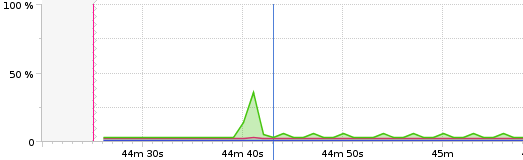
\includegraphics[width=\linewidth]{Chart--CPU-time_1.png}
    \caption{CPU usage for stress test 1: control test}
    \label{fig:CPU1}
\end{figure}

\begin{figure}[htbp]
    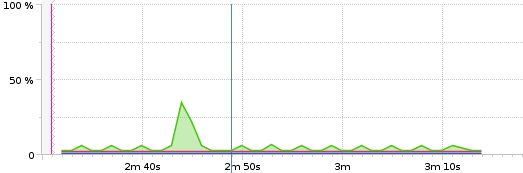
\includegraphics[width=\linewidth]{Chart--CPU-time_2.png}
    \caption{CPU usage for stress test 2: test with database containing 11,000 bank accounts}
    \label{fig:CPU2}
\end{figure}

\begin{figure}[htbp]
    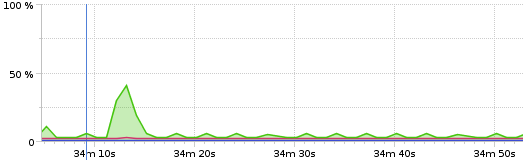
\includegraphics[width=\linewidth]{Chart--CPU-time_3.png}
    \caption{CPU usage for stress test 3: test with database containing 11,000 bank accounts and 10,000 transactions}
    \label{fig:CPU3}
\end{figure}


\begin{figure}[htbp]
    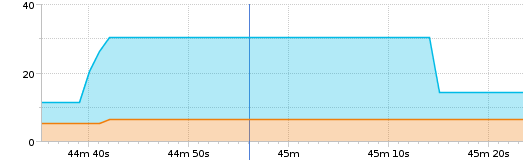
\includegraphics[width=\linewidth]{Chart--Threads_1.png}
    \caption{Thread count for stress test 1: control test}
    \label{fig:Thread1}
\end{figure}

\begin{figure}[htbp]
    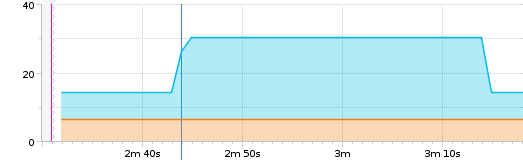
\includegraphics[width=\linewidth]{Chart--Threads_2.png}
    \caption{Thread count for stress test 2: test with database containing 11,000 bank accounts}
    \label{fig:Thread2}
\end{figure}

\begin{figure}[htbp]
    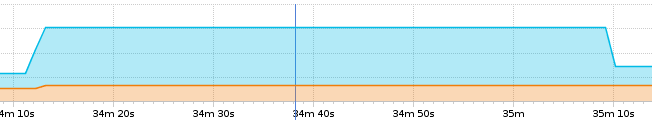
\includegraphics[width=\linewidth]{Chart--Threads_3.png}
    \caption{Thread count for stress test 3: test with database containing 11,000 bank accounts and 10,000 transactions}
    \label{fig:Thread3}
\end{figure}

\clearpage

\begin{longtable}{|m{4cm}|l|}
\hline
\cellcolor[HTML]{C0C0C0}\textbf{Tester Name} & \multicolumn{1}{p{13cm}|}{Anne-Laure}\\ \hline
\cellcolor[HTML]{C0C0C0}\textbf{Test Date} & \multicolumn{1}{p{13cm}|}{5/4/18}\\ \hline
\cellcolor[HTML]{C0C0C0}\textbf{Purpose} & \multicolumn{1}{p{13cm}|}{This test suite contains the series of tests performed with yourKit Java Profiler.}\\ \hline
\multicolumn{2}{|l|}{\cellcolor[HTML]{C0C0C0}\textbf{System specification}}\\ \hline
\cellcolor[HTML]{C0C0C0}\textbf{OS} & \multicolumn{1}{p{13cm}|}{GNU/Linux Fedora 27 x64, version 4.13.9-300}\\ \hline
\cellcolor[HTML]{C0C0C0}\textbf{RAM} & \multicolumn{1}{p{13cm}|}{4GB}\\ \hline
\cellcolor[HTML]{C0C0C0}\textbf{Graphics Card} & \multicolumn{1}{p{13cm}|}{Intel Celeron 3205U @ 1.50GHz x 2}\\ \hline
\cellcolor[HTML]{C0C0C0}\textbf{OpenJDK version} & \multicolumn{1}{p{13cm}|}{1.8.0\_144}\\ \hline
\cellcolor[HTML]{C0C0C0}\textbf{Profiler} & \multicolumn{1}{p{13cm}|}{YourKit Java Profiler 2017.02-b75}\\ \hline
\end{longtable}

\begin{longtable}{|m{4cm}|l|}
\hline
\multicolumn{2}{|l|}{control stress test: local database with 5 accounts and 5 transactions}\\ \hline
\cellcolor[HTML]{C0C0C0}\textbf{CPU usage chart} & \multicolumn{1}{p{13cm}|}{CPU usage chart 1}\\ \hline
\cellcolor[HTML]{C0C0C0}\textbf{Thread Count chart} & \multicolumn{1}{p{13cm}|}{Thread Count chart 1}\\ \hline
\cellcolor[HTML]{C0C0C0}\textbf{Events} & \multicolumn{1}{p{13cm}|}{\begin{tabular}[c]{@{}l@{}}44m 38s: application launched\\ 44m 40s: login menu loaded\\ 44m 45s: logged in\\ 44m 47s: sorted accounts by type\\ 44m 53s: removed bank account 2\\ 44m 58s: added back account 2\\ 45m 02s: viewed all transactions\\ 45m 15s: shut down application\\ \end{tabular}}\\ \hline
\end{longtable}

\begin{tabularx}{18cm}{  |*{6}{Y|} }
\cline{1-6}\multicolumn{6}{|c|}{\cellcolor[HTML]{C0C0C0}\textbf{Memory}}\\ \hline
\multicolumn{3}{|c|}{\cellcolor[HTML]{C0C0C0}\textbf{Heap-Memory}}
& \multicolumn{3}{|c|}{\cellcolor[HTML]{C0C0C0}\textbf{Non-Heap Memory}}\\ \hline
\cellcolor[HTML]{C0C0C0}\textbf{Used}
& \cellcolor[HTML]{C0C0C0}\textbf{Allocated}
& \cellcolor[HTML]{C0C0C0}\textbf{Limit}
& \cellcolor[HTML]{C0C0C0}\textbf{Used}
& \cellcolor[HTML]{C0C0C0}\textbf{Allocated}
& \cellcolor[HTML]{C0C0C0}\textbf{Limit} \\\hline
73MB
& 140MB
& 910MB
& 65 MB
& 65 MB
& 65 MB\\ \hline
\end{tabularx}
\begin{tabularx}{18cm}{  |*{5}{Y|} }
\cline{1-5}\multicolumn{5}{|c|}{\cellcolor[HTML]{C0C0C0}\textbf{CPU}}\\ \hline
\multicolumn{1}{|c|}{\cellcolor[HTML]{C0C0C0}\textbf{Classes}}
& \multicolumn{4}{|c|}{\cellcolor[HTML]{C0C0C0}\textbf{Threads}}\\ \hline
\multirow{2}{*}{8,415}& \cellcolor[HTML]{C0C0C0}\textbf{Currently live}
& \cellcolor[HTML]{C0C0C0}\textbf{Currently live daemons}
& \cellcolor[HTML]{C0C0C0}\textbf{Peak}
& \cellcolor[HTML]{C0C0C0}\textbf{Total created} \\
\cline{2-5}& 11
& 5
& 31
& 53\\ \hline
\end{tabularx}
\break \break \break
\begin{longtable}{|m{4cm}|l|}
\hline
\multicolumn{2}{|l|}{stress test: local database with 11,000 accounts and 5 transactions}\\ \hline
\cellcolor[HTML]{C0C0C0}\textbf{CPU usage chart} & \multicolumn{1}{p{13cm}|}{CPU usage chart 2}\\ \hline
\cellcolor[HTML]{C0C0C0}\textbf{Thread Count chart} & \multicolumn{1}{p{13cm}|}{Thread Count chart 2}\\ \hline
\cellcolor[HTML]{C0C0C0}\textbf{Events} & \multicolumn{1}{p{13cm}|}{\begin{tabular}[c]{@{}l@{}}2m 43s: application launched\\ 2m 46s: login menu loaded\\ 2m 51s: logged in\\ 2m 52s: sorted accounts by type\\ 2m 53s: reversed sort of accounts by type\\ 2m 54s: sorted accounts by ID\\ 2m 55s: clicked on an account to view account details\\ 2m 57s: returned to account list\\ 3m 02s: viewed all transactions\\ 3m 15s: shut down application\\ \end{tabular}}\\ \hline
\end{longtable}

\begin{tabularx}{18cm}{  |*{6}{Y|} }
\cline{1-6}\multicolumn{6}{|c|}{\cellcolor[HTML]{C0C0C0}\textbf{Memory}}\\ \hline
\multicolumn{3}{|c|}{\cellcolor[HTML]{C0C0C0}\textbf{Heap-Memory}}
& \multicolumn{3}{|c|}{\cellcolor[HTML]{C0C0C0}\textbf{Non-Heap Memory}}\\ \hline
\cellcolor[HTML]{C0C0C0}\textbf{Used}
& \cellcolor[HTML]{C0C0C0}\textbf{Allocated}
& \cellcolor[HTML]{C0C0C0}\textbf{Limit}
& \cellcolor[HTML]{C0C0C0}\textbf{Used}
& \cellcolor[HTML]{C0C0C0}\textbf{Allocated}
& \cellcolor[HTML]{C0C0C0}\textbf{Limit} \\\hline
123MB
& 203MB
& 910MB
& 67 MB
& 67 MB
& 67 MB\\ \hline
\end{tabularx}
\begin{tabularx}{18cm}{  |*{5}{Y|} }
\cline{1-5}\multicolumn{5}{|c|}{\cellcolor[HTML]{C0C0C0}\textbf{CPU}}\\ \hline
\multicolumn{1}{|c|}{\cellcolor[HTML]{C0C0C0}\textbf{Classes}}
& \multicolumn{4}{|c|}{\cellcolor[HTML]{C0C0C0}\textbf{Threads}}\\ \hline
\multirow{2}{*}{8,454}& \cellcolor[HTML]{C0C0C0}\textbf{Currently live}
& \cellcolor[HTML]{C0C0C0}\textbf{Currently live daemons}
& \cellcolor[HTML]{C0C0C0}\textbf{Peak}
& \cellcolor[HTML]{C0C0C0}\textbf{Total created} \\
\cline{2-5}& 14
& 6
& 31
& 48\\ \hline
\end{tabularx}
\break \break \break
\begin{longtable}{|m{4cm}|l|}
\hline
\multicolumn{2}{|l|}{stress test: local database with 11,000 accounts and 10,000 transactions}\\ \hline
\cellcolor[HTML]{C0C0C0}\textbf{CPU usage chart} & \multicolumn{1}{p{13cm}|}{CPU usage chart 2}\\ \hline
\cellcolor[HTML]{C0C0C0}\textbf{Thread Count chart} & \multicolumn{1}{p{13cm}|}{Thread Count chart 2}\\ \hline
\cellcolor[HTML]{C0C0C0}\textbf{Events} & \multicolumn{1}{p{13cm}|}{\begin{tabular}[c]{@{}l@{}}34m 11s: application launched\\ 34m 14s: login menu loaded\\ 34m 18s: logged in\\ 34m 20s: sorted accounts by type\\ 34m 25s: reversed sort of accounts by type\\ 34m 27s: sorted accounts by ID\\ 34m 29s: clicked on an account to view account details\\ 34m 30s: returned to account list\\ 34m 34s: viewed all transactions\\ 34m 37s: returned to account list\\ 35m 1s: shut down application\\ \end{tabular}}\\ \hline
\end{longtable}

\begin{tabularx}{18cm}{  |*{6}{Y|} }
\cline{1-6}\multicolumn{6}{|c|}{\cellcolor[HTML]{C0C0C0}\textbf{Memory}}\\ \hline
\multicolumn{3}{|c|}{\cellcolor[HTML]{C0C0C0}\textbf{Heap-Memory}}
& \multicolumn{3}{|c|}{\cellcolor[HTML]{C0C0C0}\textbf{Non-Heap Memory}}\\ \hline
\cellcolor[HTML]{C0C0C0}\textbf{Used}
& \cellcolor[HTML]{C0C0C0}\textbf{Allocated}
& \cellcolor[HTML]{C0C0C0}\textbf{Limit}
& \cellcolor[HTML]{C0C0C0}\textbf{Used}
& \cellcolor[HTML]{C0C0C0}\textbf{Allocated}
& \cellcolor[HTML]{C0C0C0}\textbf{Limit} \\\hline
158MB
& 207MB
& 910MB
& 70 MB
& 70 MB
& 70 MB\\ \hline
\end{tabularx}
\begin{tabularx}{18cm}{  |*{5}{Y|} }
\cline{1-5}\multicolumn{5}{|c|}{\cellcolor[HTML]{C0C0C0}\textbf{CPU}}\\ \hline
\multicolumn{1}{|c|}{\cellcolor[HTML]{C0C0C0}\textbf{Classes}}
& \multicolumn{4}{|c|}{\cellcolor[HTML]{C0C0C0}\textbf{Threads}}\\ \hline
\multirow{2}{*}{8,456}& \cellcolor[HTML]{C0C0C0}\textbf{Currently live}
& \cellcolor[HTML]{C0C0C0}\textbf{Currently live daemons}
& \cellcolor[HTML]{C0C0C0}\textbf{Peak}
& \cellcolor[HTML]{C0C0C0}\textbf{Total created} \\
\cline{2-5}& 14
& 6
& 31
& 88\\ \hline
\end{tabularx}
\break \break \break



\textit{Responsiveness}

Finally, the series of tests performed for responsiveness. Here, we used stopwatch testing, where each call and return to a service is logged by a stopwatch (the stopwatch used is from java's standard library). We ran these functions a multitude of times, and computed the average computing time for each method. We also averaged those for each class, and computed the average computing time for all functions in a specific class. We notice here that the connection to the database is extremely fast even on a fairly underpowered computer, with all database functions staying under half a second. The only function that fails the performance requirement (staying under 2 seconds of computing time) here is the send email function, however, this is due to the overhead incurred by the email library that we use, by the fact that the email is sent over the internet. Hence, we consider that we have met 90\% of the performance non-functional requirement as set in the requirements specification.

\begin{longtable}{|m{4cm}|l|}
\hline
\cellcolor[HTML]{C0C0C0}\textbf{Tester Name} & \multicolumn{1}{p{13cm}|}{Anne-Laure}\\ \hline
\cellcolor[HTML]{C0C0C0}\textbf{Test Date} & \multicolumn{1}{p{13cm}|}{7/4/18}\\ \hline
\cellcolor[HTML]{C0C0C0}\textbf{Purpose} & \multicolumn{1}{p{13cm}|}{This test suite contains the average time of lengths obtained through stopwatch testing.}\\ \hline
\multicolumn{2}{|l|}{\cellcolor[HTML]{C0C0C0}\textbf{System specification}}\\ \hline
\end{longtable}

\begin{longtable}{|m{9cm}|l|}
\hline
\cellcolor[HTML]{C0C0C0}\textbf{Service method} & \multicolumn{1}{p{8cm}|}{\cellcolor[HTML]{C0C0C0}\textbf{Time in seconds}}\\ \hline
\cellcolor[HTML]{C0C0C0}\textbf{EmailService:sendEmail} & \multicolumn{1}{p{8cm}|}{5.88586}\\ \hline
\cellcolor[HTML]{C0C0C0}\textbf{CSVGenerator:generateCSV} & \multicolumn{1}{p{8cm}|}{0.015645}\\ \hline
\cellcolor[HTML]{C0C0C0}\textbf{UserService:deleteBankAccount} & \multicolumn{1}{p{8cm}|}{0.377784}\\ \hline
\cellcolor[HTML]{C0C0C0}\textbf{AccountService:addAccount} & \multicolumn{1}{p{8cm}|}{0.21009}\\ \hline
\cellcolor[HTML]{C0C0C0}\textbf{UserService:updateUser} & \multicolumn{1}{p{8cm}|}{0.022402}\\ \hline
\cellcolor[HTML]{C0C0C0}\textbf{ConnectionProvider:getConnectionSource} & \multicolumn{1}{p{8cm}|}{0.187765}\\ \hline
\end{longtable}

\begin{longtable}{|m{9cm}|l|}
\hline
\cellcolor[HTML]{C0C0C0}\textbf{Service class} & \multicolumn{1}{p{8cm}|}{\cellcolor[HTML]{C0C0C0}\textbf{Time in seconds}}\\ \hline
\cellcolor[HTML]{C0C0C0}\textbf{UserService} & \multicolumn{1}{p{8cm}|}{0.400186}\\ \hline
\cellcolor[HTML]{C0C0C0}\textbf{CSVGenerator} & \multicolumn{1}{p{8cm}|}{0.015645}\\ \hline
\cellcolor[HTML]{C0C0C0}\textbf{AccountService} & \multicolumn{1}{p{8cm}|}{0.21009}\\ \hline
\cellcolor[HTML]{C0C0C0}\textbf{ConnectionProvider} & \multicolumn{1}{p{8cm}|}{0.187765}\\ \hline
\cellcolor[HTML]{C0C0C0}\textbf{EmailService} & \multicolumn{1}{p{8cm}|}{5.88586}\\ \hline
\end{longtable}





\section{Acceptance Testing}
\subsubsection{Create User Account}
\begin{longtable}{|m{4cm}|l|l|} 
\caption[]{Create User Account} 
\hline 
\cellcolor[HTML]{C0C0C0}\textbf{Use Case} & \multicolumn{2}{p{13cm}|}{Create User Account}\\ \hline
\cellcolor[HTML]{C0C0C0}\textbf{Description} & \multicolumn{2}{p{13cm}|}{As a user, I would like to be able to create an account}\\ \hline
\cellcolor[HTML]{C0C0C0}\textbf{Description} & \multicolumn{2}{p{13cm}|}{\begin{tabular}[c]{@{}l@{}}$\bullet$ The create account button is visible and easy to find\\ $\bullet$ Clear error codes were shown when errors were inputted\\ $\bullet$ The processing is fast enough\\ \end{tabular}}\\ \hline
\end{longtable}



\section{Installation Testing}
\subsubsection{Installation: Linux}
\begin{longtable}{|m{4cm}|l|l|} 
\caption[]{Linux} 
\hline 
\cellcolor[HTML]{C0C0C0}\textbf{Operating System} & \multicolumn{2}{p{13cm}|}{Linux}\\ \hline
\cellcolor[HTML]{C0C0C0}\textbf{Requirements} & \multicolumn{2}{p{13cm}|}{\begin{tabular}[c]{@{}l@{}}$\bullet$ Java 8 or higher\\ $\bullet$ 1GB of RAM or more\\ $\bullet$ Intel Celeron 3205U @ 1.50GHz x 2 or better\\ $\bullet$ 50 MB of hard disk space\\ $\bullet$ Ubuntu 12.04 LTS or newer\\ $\bullet$ Internet connectivity required to download the zip file\\ $\bullet$ Internet connectivity required to send statements by email\\ \end{tabular}}\\ \hline
\cellcolor[HTML]{C0C0C0}\textbf{Installation} & \multicolumn{2}{p{13cm}|}{\begin{tabular}[c]{@{}l@{}}$\bullet$ Download the zip file\\ $\bullet$ Extract the zip file in the location you would like to install the system\\ $\bullet$ Open up a terminal in that directory and run: java -jar MyMoney.jar\\ \end{tabular}}\\ \hline
\multicolumn{3}{|l|}{\cellcolor[HTML]{C0C0C0}\textbf{Functionalities tested}}\\ \hline
\cellcolor[HTML]{C0C0C0}\textbf{Application runs} & \multicolumn{2}{p{13cm}|}{valid}\\ \hline 
\cellcolor[HTML]{C0C0C0}\textbf{Entering user input} & \multicolumn{2}{p{13cm}|}{valid}\\ \hline 
\cellcolor[HTML]{C0C0C0}\textbf{Writing to database} & \multicolumn{2}{p{13cm}|}{valid}\\ \hline 
\cellcolor[HTML]{C0C0C0}\textbf{Saving database} & \multicolumn{2}{p{13cm}|}{valid}\\ \hline 
\cellcolor[HTML]{C0C0C0}\textbf{Exporting CSV statement} & \multicolumn{2}{p{13cm}|}{valid}\\ \hline 
\cellcolor[HTML]{C0C0C0}\textbf{Emailing CSV statement} & \multicolumn{2}{p{13cm}|}{valid}\\ \hline 
\end{longtable}

\subsubsection{Installation: MacOS}
\begin{longtable}{|m{4cm}|l|l|} 
\caption[]{MacOS} 
\hline 
\cellcolor[HTML]{C0C0C0}\textbf{Operating System} & \multicolumn{2}{p{13cm}|}{MacOS}\\ \hline
\cellcolor[HTML]{C0C0C0}\textbf{Requirements} & \multicolumn{2}{p{13cm}|}{\begin{tabular}[c]{@{}l@{}}$\bullet$ Java 8 or higher\\ $\bullet$ 1GB of RAM or more\\ $\bullet$ Intel Celeron 3205U @ 1.50GHz x 2 or better\\ $\bullet$ 50 MB of hard disk space\\ $\bullet$ MacOS 10.8 or newer\\ $\bullet$ Internet connectivity required to download the zip file\\ $\bullet$ Internet connectivity required to send statements by email\\ \end{tabular}}\\ \hline
\cellcolor[HTML]{C0C0C0}\textbf{Installation} & \multicolumn{2}{p{13cm}|}{\begin{tabular}[c]{@{}l@{}}$\bullet$ Download the zip file\\ $\bullet$ Extract the zip file in the location you would like to install the system\\ $\bullet$ Open up a terminal in that directory and run: java -jar MyMoney.jar\\ \end{tabular}}\\ \hline
\multicolumn{3}{|l|}{\cellcolor[HTML]{C0C0C0}\textbf{Functionalities tested}}\\ \hline
\cellcolor[HTML]{C0C0C0}\textbf{Application runs} & \multicolumn{2}{p{13cm}|}{valid}\\ \hline 
\cellcolor[HTML]{C0C0C0}\textbf{Entering user input} & \multicolumn{2}{p{13cm}|}{valid}\\ \hline 
\cellcolor[HTML]{C0C0C0}\textbf{Writing to database} & \multicolumn{2}{p{13cm}|}{valid}\\ \hline 
\cellcolor[HTML]{C0C0C0}\textbf{Saving database} & \multicolumn{2}{p{13cm}|}{valid}\\ \hline 
\cellcolor[HTML]{C0C0C0}\textbf{Exporting CSV statement} & \multicolumn{2}{p{13cm}|}{valid}\\ \hline 
\cellcolor[HTML]{C0C0C0}\textbf{Emailing CSV statement} & \multicolumn{2}{p{13cm}|}{valid}\\ \hline 
\end{longtable}

\subsubsection{Installation: Windows}
\begin{longtable}{|m{4cm}|l|l|} 
\caption[]{Windows} 
\hline 
\cellcolor[HTML]{C0C0C0}\textbf{Operating System} & \multicolumn{2}{p{13cm}|}{Windows}\\ \hline
\cellcolor[HTML]{C0C0C0}\textbf{Requirements} & \multicolumn{2}{p{13cm}|}{\begin{tabular}[c]{@{}l@{}}$\bullet$ Java 8 or higher\\ $\bullet$ 1GB of RAM or more\\ $\bullet$ Intel Celeron 3205U @ 1.50GHz x 2 or better\\ $\bullet$ 50 MB of hard disk space\\ $\bullet$ Windows 10 or newer\\ $\bullet$ Internet connectivity required to download the zip file\\ $\bullet$ Internet connectivity required to send statements by email\\ \end{tabular}}\\ \hline
\cellcolor[HTML]{C0C0C0}\textbf{Installation} & \multicolumn{2}{p{13cm}|}{\begin{tabular}[c]{@{}l@{}}$\bullet$ Download the zip file\\ $\bullet$ Extract the zip file in the location you would like to install the system\\ $\bullet$ Open up a terminal in that directory and run: java -jar MyMoney.jar\\ \end{tabular}}\\ \hline
\multicolumn{3}{|l|}{\cellcolor[HTML]{C0C0C0}\textbf{Functionalities tested}}\\ \hline
\cellcolor[HTML]{C0C0C0}\textbf{Application runs} & \multicolumn{2}{p{13cm}|}{valid}\\ \hline 
\cellcolor[HTML]{C0C0C0}\textbf{Entering user input} & \multicolumn{2}{p{13cm}|}{valid}\\ \hline 
\cellcolor[HTML]{C0C0C0}\textbf{Writing to database} & \multicolumn{2}{p{13cm}|}{valid}\\ \hline 
\cellcolor[HTML]{C0C0C0}\textbf{Saving database} & \multicolumn{2}{p{13cm}|}{valid}\\ \hline 
\cellcolor[HTML]{C0C0C0}\textbf{Exporting CSV statement} & \multicolumn{2}{p{13cm}|}{valid}\\ \hline 
\cellcolor[HTML]{C0C0C0}\textbf{Emailing CSV statement} & \multicolumn{2}{p{13cm}|}{valid}\\ \hline 
\end{longtable}



\section{References}

\begin{itemize}
    \item Craig Larman, Applying UML and Patterns: An Introduction to Object-Oriented Analysis and Design and Iterative Development, 3rd edition, Prentice-Hall, 2005.
    \item Roger S Pressman, Software Engineering: A Practitioner's Approach, 7th edition, McGraw-Hill
    \item Greg Butler's course COMP 354 content

\end{itemize}

\appendix

\subsection*{Description of File Format: Input}

The user enters plain text through the graphical user interface of the system.

\subsection*{Description of File Format: Output}

The system displays information through the graphics user interface. The system also creates files (statements) in the user specified location
in the filesystem. The system emails the files (statements) to the user specified email address.

\end{document}
